% ---------------------------------------------------------------------------
% ---------------------------------------------------------------------------
% Modelo LaTex para preparação do documento final de Dissertação de Mestrado
% O modelo está em conformidade com ABNT NBR 14724:2011:
% Programa de Pós-Graduação em Informática
% Universidade Federal de Alagoas
% Versão: v0.9
% ---------------------------------------------------------------------------
% ---------------------------------------------------------------------------

\PassOptionsToPackage{inline}{enumitem}

\documentclass[
	% -- opções da classe memoir --
	12pt,					% tamanho da fonte
	openright,				% capítulos começam em páginas ímpares (insere página vazia caso preciso)
	oneside,				% para impressão em verso e anverso. Oposto a oneside
	a4paper,				% tamanho do papel.
	% -- opções da classe abntex2 --
	chapter=TITLE,			% títulos de capítulos convertidos em letras maiúsculas
	%section=TITLE,			% títulos de seções convertidos em letras maiúsculas
	%subsection=TITLE,		% títulos de subseções convertidos em letras maiúsculas
	%subsubsection=TITLE,	% títulos de subsubseções convertidos em letras maiúsculas
	% -- opções do pacote babel --
	english,				% idioma adicional para hifenização
	%french,				% idioma adicional para hifenização
	%spanish,				% idioma adicional para hifenização
	brazil					% o último idioma é o principal do documento
]{abntex2}

% ---------------------
% Pacotes OBRIGATÓRIOS
% ---------------------
\usepackage[T1]{fontenc}		% Seleção de códigos de fonte.
\usepackage[utf8]{inputenc}		% Codificação do documento (conversão automática dos acentos)
\usepackage{lastpage}			% Usado pela Ficha catalográfica
\usepackage{indentfirst}		% Identa o primeiro parágrafo de cada seção.
\usepackage{color}				% Controle das cores
\usepackage{graphicx,graphicx}	% Inclusão de gráficos
\usepackage{epsfig,subfig}		% Inclusão de figuras
\usepackage{microtype} 			% Melhorias de justificação
% ---------------------

% ---------------------
% Pacotes ADICIONAIS
% ---------------------
% \usepackage{lipsum}					% Geração de dummy text
\usepackage{amsmath,amssymb}	        % Comandos matemáticos avançados
\usepackage{setspace}  					% Para permitir espaçamento simples, 1 1/2 e duplo
\usepackage{verbatim}					% Para poder usar o ambiente "comment"
\usepackage{tabularx} 					% Para poder ter tabelas com colunas de largura auto-ajustável
\usepackage{afterpage} 					% Para executar um comando depois do fim da página corrente
\usepackage{url} 						% Para formatar URLs (endereços da Web)
\usepackage{svg}
\counterwithin{figure}{chapter}         % Para numerar figuras por capítulo
\usepackage{enumerate}
%\usepackage{tocloft}
%\setlength{\cftfignumwidth}{4em}% change 4em to suit
% ---------------------

% ---------------------
% Pacotes de CITAÇÕES
% ---------------------
\usepackage[brazilian,hyperpageref]{backref}  % Paginas com as citações na bibliografia
\usepackage[alf]{abntex2cite}				  % Citações padrão ABNT (alfa)
%\usepackage[num]{abntex2cite}				  % Citações padrão ABNT (numéricas)
% ---------------------

% Definição de diretório de imagens
\graphicspath{{imagens/}}

% Configurações de CITAÇÕES para abntex2
% --- 
% CONFIGURAÇÕES DE PACOTES
% --- 

% ---
% Configurações do pacote backref
% Usado sem a opção hyperpageref de backref
\renewcommand{\backrefpagesname}{Citado na~(s) página~(s):~}
% Texto padrão antes do número das páginas
\renewcommand{\backref}{}
% Define os textos da citação
\renewcommand*{\backrefalt}[4]{
	\ifcase #1 %
		Nenhuma citação no texto.%
	\or
		Citado na página #2.%
	\else
		Citado #1 vezes nas páginas #2.%
	\fi}%
% ---

% Inclusão de dados para CAPA e FOLHA DE ROSTO (título, autor, orientador, etc.)
% ---
% Informações de dados para CAPA e FOLHA DE ROSTO
% ---
\titulo{FRAMEWORK COMPUTACIONAL PARA ANÁLISE DE FADIGA EM DUTOS SUBMARINOS EM VÃO-LIVRE}
\autor{Weverton Marques da Silva}
\local{Maceió-AL}
\data{Dezembro de 2020}
\orientador{Adeildo Soares Ramos Júnior}
\coorientador{Eduardo Setton S. da Silveira}
\instituicao{%
  Universidade Federal de Alagoas --- UFAL
  \par
  Centro de Tecnologia
  \par
  Programa de Pós-Graduação em Engenharia Civil
}
\tipotrabalho{Dissertação (Mestrado)}
% O preambulo deve conter o tipo do trabalho, o objetivo,
% o nome da instituição e a área de concentração
\preambulo{Dissertação apresentada como requisito parcial para obtenção do grau de Mestre pelo Programa de Pós-Graduação em Engenharia Civil do Centro de Tecnologia da Universidade Federal de Alagoas.}
% ---


% Inclui Configurações de aparência do PDF Final
%  Configurações de aparência do PDF final
% NÃO ALTERAR!!!

% alterando o aspecto da cor azul
\definecolor{blue}{RGB}{41,5,195}

% informações do PDF
\makeatletter
\hypersetup{
     	%pagebackref=true,
		pdftitle={\@title}, 
		pdfauthor={\@author},
    		pdfsubject={\imprimirpreambulo},
	    pdfcreator={LaTeX with abnTeX2},
		pdfkeywords={abnt}{latex}{abntex}{abntex2}{trabalho acadêmico}, 
		colorlinks=true,       		% false: boxed links; true: colored links
    		linkcolor=black,          	% color of internal links
    		citecolor=black,        		% color of links to bibliography
    		filecolor=black,      		% color of file links
		urlcolor=black,
		bookmarksdepth=4
} 
\makeatother
% --- 

% Inclui configurações da folha de rosto
\renewcommand{\folhaderostocontent}{
	\begin{center}
		\MakeUppercase{\imprimirautor}
		
		\vspace*{\fill}
		\vspace*{\fill}
		\textbf{\imprimirtitulo}
		
		\vspace*{\fill}
		\hspace{.45\textwidth}
		\begin{minipage}{.5\textwidth}
			\SingleSpacing
			\imprimirpreambulo
			
			\vspace*{1cm}
			\imprimirorientadorRotulo~\imprimirorientador
			\par
			\imprimircoorientadorRotulo~\imprimircoorientador
		\end{minipage}
		
		\vspace*{\fill}
		\vspace*{\fill}
		\imprimirlocal
		\par
		\imprimirdata
	\end{center}
}


% Configurações da fonte do texto
\usepackage{times}						% Usar a fonte Times New Roman
\renewcommand{\ABNTEXpartfontsize}{\normalsize}
\renewcommand{\ABNTEXsectionfontsize}{\normalsize}
\renewcommand{\ABNTEXsubsectionfontsize}{\normalsize}
\renewcommand{\ABNTEXsubsubsectionfontsize}{\normalsize}
\renewcommand{\ABNTEXsubsubsubsectionfontsize}{\normalsize}
\renewcommand{\ABNTEXchapterfontsize}{\normalsize}

%\chapterstyle{article}
\renewcommand{\ABNTEXchapterfont}{\fontseries{b}}

% O tamanho da identação do parágrafo é dado por:
\setlength{\parindent}{1.3cm}

% Controle do espaçamento entre um parágrafo e outro:
\setlength{\parskip}{0.2cm}  % tente também \onelineskip

% Espaço entre o título do capítulo e o texto
\setlength{\afterchapskip}{0.8cm}

% ---------------------
% Compila o índice
% ---------------------
\makeindex
% ---------------------

%%%%%%%%%%%%%%%%%%%%%%%%%%%
%%  INICIO DO DOCUMENTO  %%
%%%%%%%%%%%%%%%%%%%%%%%%%%%
\begin{document}

% Elementos textuais com numeração arábica
\pagenumbering{arabic}

% Retira espaço extra obsoleto entre as frases.
\frenchspacing

% ----------------------------------------------------------
% ELEMENTOS PRÉ-TEXTUAIS (Capa, Resumo, Abstract, etc.)
% ----------------------------------------------------------
\pretextual

% Capa
% ---
% Impressão da Capa
% ---
\begin{capa}
	\center
	UNIVERSIDADE FEDERAL DE ALAGOAS\\
	CENTRO DE TECNOLOGIA\\
	PROGRAMA DE PÓS GRADUAÇÃO EM ENGENHARIA CIVIL

	\vfill
	\MakeUppercase{\imprimirautor}

    \vfill
    \textbf{\imprimirtitulo}
    \vfill
    \vfill
    \imprimirlocal
    \par
    \imprimirdata

    \vspace*{1cm}
\end{capa}
% ---

% Folha de rosto (o * indica que haverá a ficha bibliográfica)
\imprimirfolhaderosto

% Imprimir Ficha Catalográfica
%% ---
% Ficha Catalográfica
% ---
% Isto é um exemplo de Ficha Catalográfica, ou ``Dados internacionais de
% catalogação-na-publicação''. Você pode utilizar este modelo como referência.
% Porém, provavelmente a biblioteca da sua universidade lhe fornecerá um PDF
% com a ficha catalográfica definitiva após a defesa do trabalho. Quando estiver
% com o documento, salve-o como PDF no diretório do seu projeto e substitua todo
% o conteúdo de implementação deste arquivo pelo comando abaixo:
%
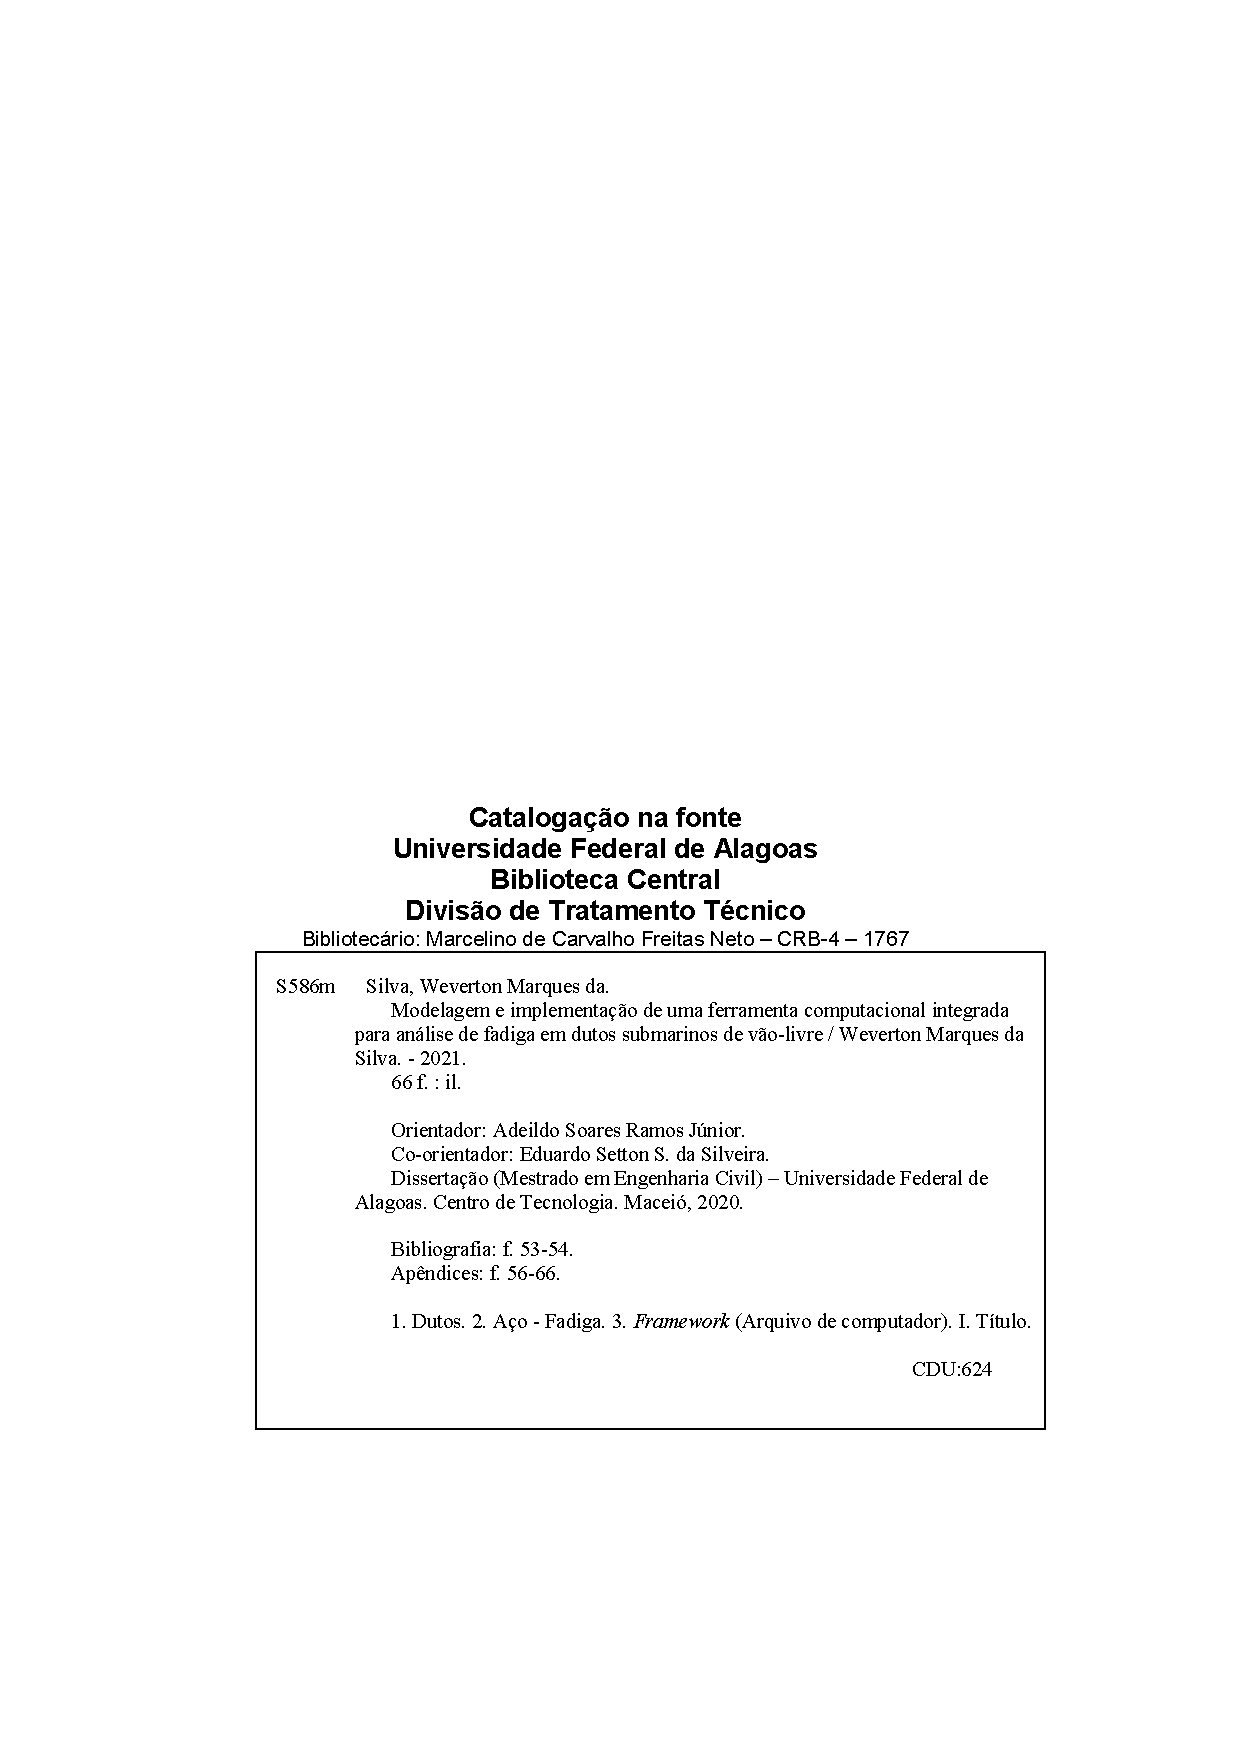
\includepdf{pretextual/ficha_catalografica.pdf}

% Inserir Folha de Aprovação
%% ---
% Assinaturas
% ---
% Isto é um exemplo de Folha de aprovação, elemento obrigatório da NBR
% 14724/2011 (seção 4.2.1.3). Você pode utilizar este modelo até a aprovação
% do trabalho. Após isso, substitua todo o conteúdo deste arquivo por uma
% imagem da página assinada pela banca com o comando abaixo:
%
% \includepdf{folhadeaprovacao_final.pdf}
%
\begin{folhadeaprovacao}
	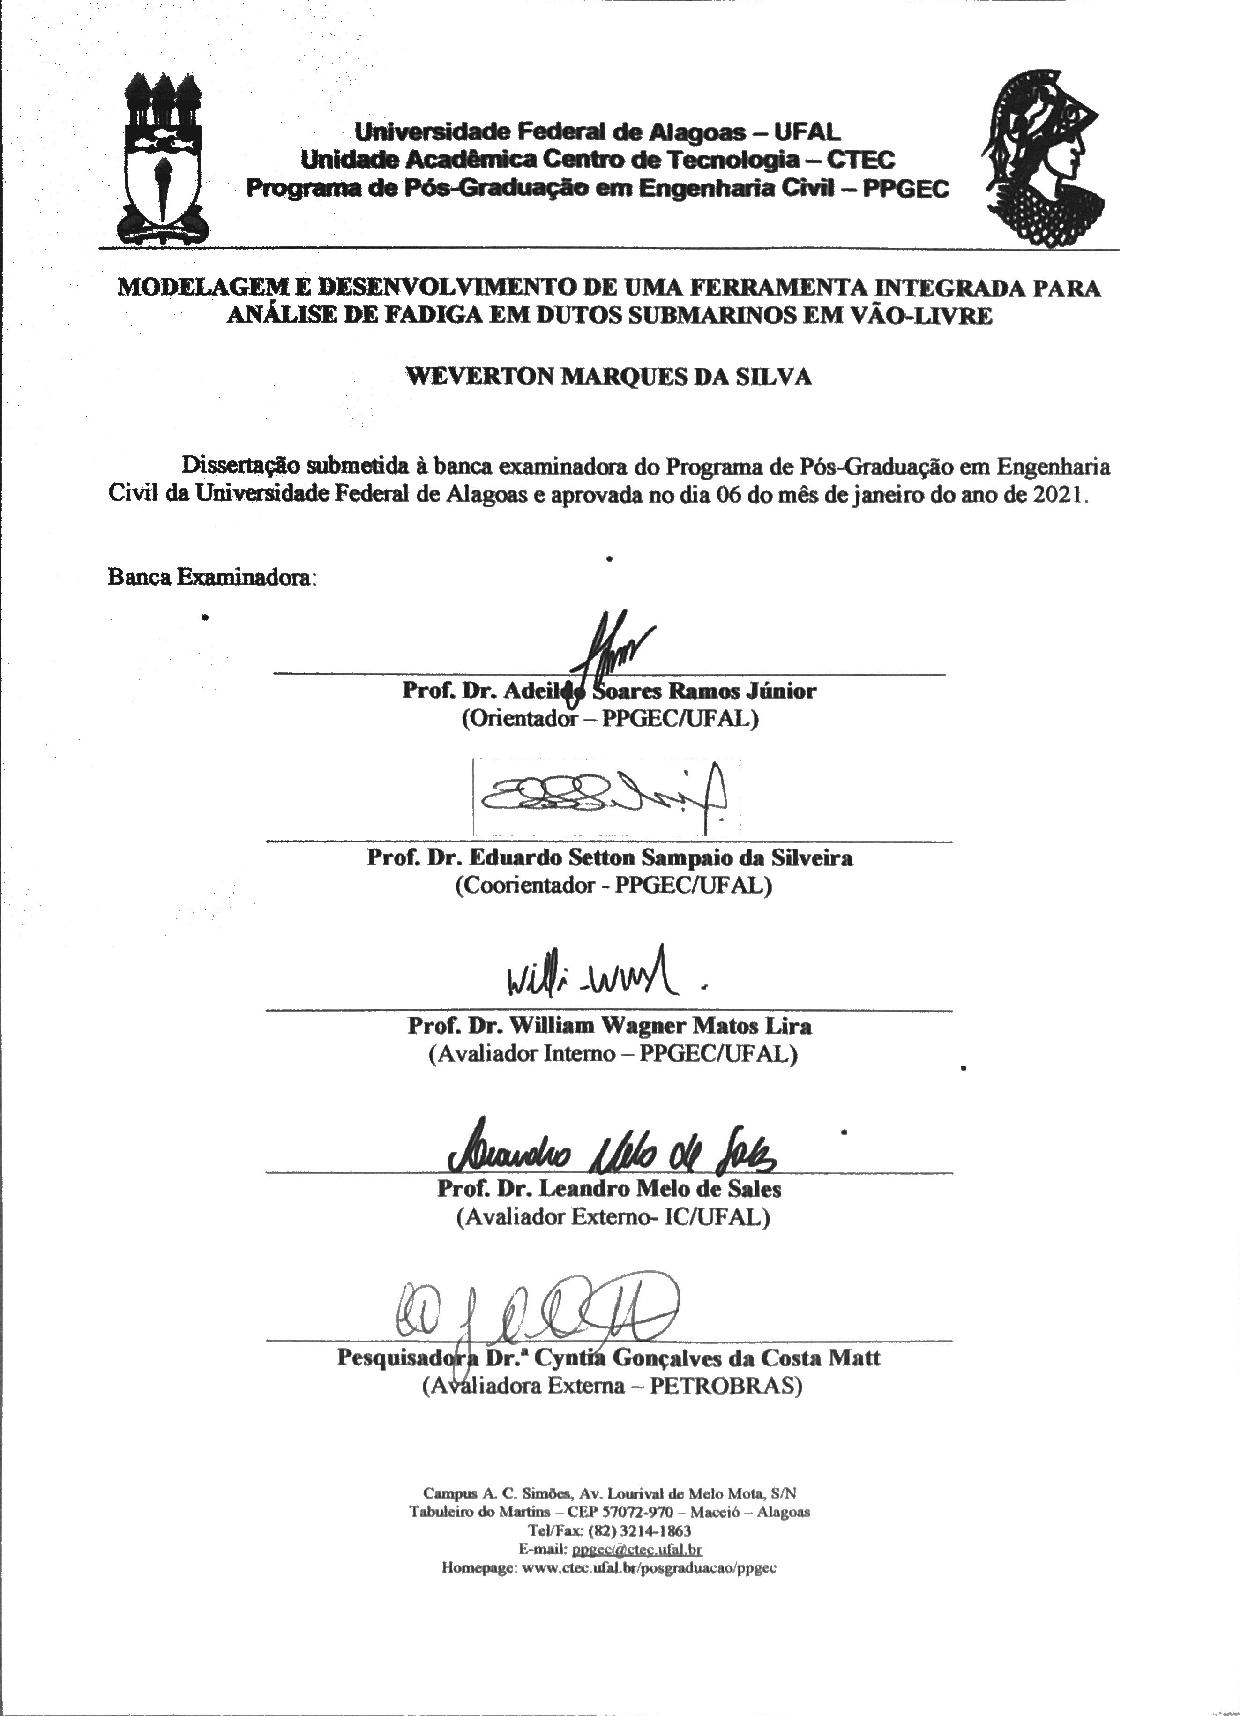
\includepdf{pretextual/folha_de_aprovacao}
	% \begin{center}
	% 	\textbf{Folha de Aprovação}
	% 	\vfill

	% 	AUTOR: \MakeUppercase{\imprimirautor}

	% 	\vfill
	% 	\imprimirtitulo
	% 	\vfill

	% 	\hspace{.45\textwidth}
	% 	\begin{minipage}{.5\textwidth}
	% 		\imprimirpreambulo
	% 	\end{minipage}%
	% 	\vfill

	% 	Trabalho aprovado. \imprimirlocal, 28 de setembro de 2016:
	% \end{center}

	% \assinatura{\textbf{\imprimirorientador} \\ Orientador}
	% \assinatura{\textbf{\imprimircoorientador} \\ Co-Orientador}
	% \assinatura{\textbf{William Wagner Matos Lira} \\ Convidado 1}
	% \assinatura{\textbf{Leandro Melo de Sales} \\ Convidado 2}

\end{folhadeaprovacao}

% Dedicatória
%% ---
% Dedicatória
% ---
\begin{dedicatoria}
   \vspace*{\fill}
   \centering
   \noindent
   \textit{ Aos meus pais XXXXXXXX e YYYYYYY, \\ por sempre estarem comigo em todos os momentos.} \vspace*{\fill}
\end{dedicatoria}
% ---

% Agradecimentos
%% ---
% Agradecimentos
% ---
\begin{agradecimentos}

Aos meus familiares por todo apoio. Especialmente, ao meus irmão, Wagner, e a minha noiva, Jhulia, que estiveram sempre ao meu lado e me ajudaram a encontrar a disposição para seguir em frente.

Agradeço ao meu orientador e coorientador pelos direcionamentos e por acreditaram na importância dos frutos desse trabalho.

Ao Laboratório de Computação Científica e Visualização pela minha participação no projeto IntegriSpan. Especialmente aos meus amigos Emerson, Josué, Jéssica e Renato. Sem a ajuda e parceria inestimável deles este trabalho não seria possível.

Aos professores do Programa de Pós-Graduação em Engenharia Civil que, com os conhecimentos transmitidos nas disciplinas, me ajudaram a elaborar esse trabalho.

\end{agradecimentos}
%% ---

% Epígrafe
%% ---
% Epígrafe
% ---
\begin{epigrafe}
    \vspace*{\fill}
	\begin{flushright}
		\textit{``Seja curioso. Leia muito. Experimente coisas novas.\\ Eu acho que muito do que as pessoas chamam de inteligência\\apenas se resume a curiosidade.''\\ % chktex 38
		          (Aaron Swartz)}
	\end{flushright}
\end{epigrafe}
% ---

% Resumo e Abstract
% ---
% RESUMOS
% ---

% RESUMO em português
\setlength{\absparsep}{18pt} % ajusta o espaçamento dos parágrafos do resumo
\begin{resumo}
TODO.

 \textbf{Palavras-chaves}: TODO.
\end{resumo}

% ABSTRACT in english
\begin{resumo}[Abstract]
 \begin{otherlanguage*}{english}
   TODO.

   \vspace{\onelineskip}
 
   \noindent 
   \textbf{Keywords}: TODO.
 \end{otherlanguage*}
\end{resumo}

% Lista de ilustrações
\pdfbookmark[0]{\listfigurename}{lof}
\listoffigures*
\cleardoublepage

% Lista de tabelas
\pdfbookmark[0]{\listtablename}{lot}
\listoftables*
\cleardoublepage

% Lista de abreviaturas e siglas
\begin{siglas}
 	\item[MEF] Método dos Elementos Finitos
	\item[VIV] Vibração Induzida por Vórtice
\end{siglas}

% Lista de símbolos
%\begin{simbolos}
%  \item[$ \Gamma $] Letra grega Gama
%  \item[$ \Lambda $] Lambda
%  \item[$ \zeta $] Letra grega minúscula zeta
%  \item[$ \in $] Pertence
%\end{simbolos}

% Inserir o SUMÁRIO
\pdfbookmark[0]{\contentsname}{toc}
\tableofcontents*
\cleardoublepage

% ----------------------------------------------------------
% ELEMENTOS TEXTUAIS (Capítulos)
% ----------------------------------------------------------
\textual

% Ajusta o header para conter apenas o número da página
% \pagestyle{simple}

% Atalhos para escritas comuns
\def\integrispan{IntegriSpan}
\def\integridutos{IntegriDutos}
\def\fatfree{FatFree}
\def\dnvf105{DNVGL-RP-F105}
\def\abaqus{Abaqus}
\def\petrobras{Petrobras}

% ----------------------------------------------------------
% TEXTO DA DISSERTAÇÃO
% ----------------------------------------------------------
%\chapter{Introdução}


Ao longo das últimas décadas, à medida que novos campos de petróleo e gás foram descobertos em águas profundas e distantes da costa, surgiu a necessidade de aplicação de sistemas de coleta e exportação submarinos utilizando dutos rígidos cada vez mais extensos, e consequentemente com maior propensão à ocorrência de vãos livres induzidos por irregularidades do piso marinho.

A configuração de dutos no fundo do mar depende das características topográficas do fundo do mar, tipo de solo, tensão residual, rigidez do tubo e seu peso submerso. Seções de tubo não suportadas pelo do fundo do mar são chamadas de vãos. Se o fundo do mar for muito irregular, os dutos tendem a formar vãos em vez de seguir as características topográficas do fundo do mar. Os vãos podem ser criados devido a irregularidades no fundo do mar durante a instalação ou aos subsequentes movimentos horizontais de \textit{scouring} de dutos durante a operação.

A presença de vãos no dutos no fundo do mar exige uma avaliação para determinar se é necessária uma ação corretiva para evitar danos aos mesmos. As características estáticas e dinâmicas dos vãos da dutos devem ser investigadas para garantir que o duto possa ser mantida em um estado aceitavelmente seguro. Se a segurança necessária não puder ser garantida, as ações corretivas na forma de reencaminhamento, correção de vãos, supressão do VIV e similares são usadas para garantir que os critérios de projeto relativos aos níveis de tensão e possíveis danos à fadiga devido ao VIV não sejam excedidos.

Ainda na fase de projeto, uma avaliação do perfil do fundo do mar ao longo da rota proposta pode ser realizada para identificar se é esperado que ocorram vãos da dutos. Se ocorrerem vãos de dutos, será necessário determinar onde e quanto dos vãos será calculado. Esta análise fornece previsões dos números e tamanhos dos vãos esperados.
Devido a quantidade de fatores envolvidos, o processo de lançamento de dutos é uma das tarefas mais desafiadoras, mesmo quando a rota ideal já está definida. A análise requer o uso de métodos numéricos robustos para seu tratamento.
O Método dos Elementos Finitos (MEF) é amplamente usado nessa tarefa.

De modo a representar adequadamente as condições de campo, é necessário modelar desde a etapa de instalação até a operação do duto, assim como considerar efeito de carregamentos dos diferentes valores de pressões internas e externas nas respectivas etapas.
Modelar a instalação de dutos em um \textit{software} de elementos finitos para uso geral pode ser um trabalho demorado e tedioso, principalmente devido a grandes quantidades de dados da batimetria.
Na maioria das vezes, são necessárias técnicas avançadas de \textit{script} para definir o perfil do leito marinho, selecionar a rota ideal do duto e simular o processo de assentamento~\cite{VandenAbeele2013}.

Nesse cenário, são essenciais ferramentas que auxiliem na pré e pós-processamento de dados e na automação de procedimentos. Uma ferramenta com essas características traz ganhos significativos para a produtividade e reduzem a probabilidade de erro humano. Além disso, quando essa ferramenta integra ferramentas de uso específicos (análises e visualização), pode-se reduzir atritos do fluxo de trabalhar que usa várias ferramentas de forma isolada.

\section{Objetivos}

Este trabalho tem como objetivo geral desenvolver uma ferramenta para a análise de fadiga em dutos submarinos em vãos livre, que permita um fluxo de trabalho que inclua de um software de análise de elementos finitos e uma planilha de cálculo de vida a fadiga. Além disso,este trabalho tem como objetivos específicos:

\begin{itemize}
    \item Modelar e implementar a ferramenta utilizando o paradigma da programação orientada a objetos, através da linguagem Python.
    \item Contribuir para a metodologia de análise de fadiga em dutos por meio da criação de uma metodologia de seleção de modos de vibração.
\end{itemize}
\section{Vibração induzida por vórtices em vãos livres}

Quando um fluido de baixa viscosidade encontra um obstáculo, forma-se uma camada limite. Segundo~\citet{Currie2002}, esta é uma fina camada de fluido que está sujeita aos efeitos das forças viscosas. Nesta camada a velocidade do fluxo varia rapidamente, ficando cada vez mais lenta, formando um escoamento rotacional dentro da camada limite. Para determinadas velocidades de escoamento, a camada limite se desprende do obstáculo, formando uma esteira de vórtices, conhecida como esteira de von Kármán, conforme visto na Figura~\ref{fig:jdsn-karman}. Como consequência direta do desprendimento de vórtices, surge uma força oscilatória transversal ao fluxo, que age sobre o obstáculo, resultando em oscilações verticais e horizontais~\cite{Ni}.

\begin{figure}[!hbt]
\begin{center}
\includegraphics[width=0.6\textwidth]{jdsn-karman}
\caption{Esteira de von Kármán \cite{VandenAbeele2012}.}
\label{fig:jdsn-karman} 
\end{center}
\end{figure}

\citet{Mork2003} explica que a frequência de espalhamento de vórtices é causada por um fluxo normal ao obstáculo, nesse caso, o duto em vão livre, e é governado pelo número de Strouhal, diâmetro externo e velocidade de fluxo.
O número de Strouhal pode ser obtido pela expressão $S_t = (f L) / V$, onde $f$ é a frequência de vórtices, $L$ é o comprimento característico e $V$ é a velocidade do fluxo.
Segundo~\citet{Mork2003}, quando a velocidade do fluxo alcança uma das frequências naturais da estrutura, ela começa a vibrar e estas duas vibrações se correlacionam, causando vibrações de grande amplitude e grande dano (\textit{lock-in}).

Como os dutos são geralmente modelados como cilindros, é importante entender como funciona o comportamento do fluxo de fluido ao redor dessa estrutura.
Conforme~\citet{Batchelor1967}, citado por~\citet{Sumer1995}, ao estudar vibrações de cilindros em corrente constante, inicia-se o espalhamento de vórtices quando o número de Reynolds, $R_e = (U\cdot D)/\nu$, é maior que $40$, onde $U$ é a velocidade do fluxo, $D$ é o diâmetro do cilindro e $\nu$ é a viscosidade cinemática.

O espalhamento de vórtices induz uma variação cíclica de forças no cilindro.
Assim, enquanto uma força de sustentação, \textit{lift force}, oscila à mesma frequência do espalhamento de vórtices, a força de arrasto, \textit{drag force}, oscila à duas vezes esta mesma frequência~\cite{Sumer1995}.
Estas forças oscilatórias, os vórtices, podem induzir vibrações na direção ortogonal ao fluxo, \textit{cross-flow} (CF), e na direção do fluxo, \textit{in-line} (IL), denominadas: vibrações induzidas por vórtices (VIV).

Os diversos dutos submarinos, que tem como objetivo o transporte de fluidos, seja entre o poço e a plataforma, entre plataformas etc., estão sujeitos ao fluxo intermitente de cargas ambientais.
Essas cargas, tornam-se um desafio ainda maior quando os dutos, instalados diretamente no irregular leito marinho, encontram-se em vãos livres~\cite{Fyrileiv1998}, como ilustrado na Figura~\ref{fig:jdsn-fullfrees}.

\begin{figure}[!h]
\begin{center}
\includegraphics[width=1\textwidth]{jdsn-fullfrees}
\caption{Duto em Vão livre e direções das oscilações~\cite{DNV2017}.}
\label{fig:jdsn-fullfrees}
\end{center}
\end{figure}

Porém, vãos livres não aparecem apenas quando os dutos são instalados em leito irregular, mas também quando ocorre erosão posterior (\textit{scouring}\footnote{É a erosão do solo marinho causada pela ação de ondas ou correntes. Caracteriza-se pela remoção de sedimentos com formação de cavidades ou canais.}), devido, por exemplo, a suportes artificiais.
Com o duto exposto à ondas e correntes, a parte não apoiada estará suscetível à VIV.
Caso a frequência de espalhamento alcance uma das frequências naturais do duto, esse poderá entrar em ressonância.
As excitações dinâmicas podem causar danos por fadiga, sendo importante identificar os corretos procedimentos de intervenção, seja no duto ou no leito marinho.

A \dnvf105 utiliza uma metodologia baseada em modelos de resposta para avaliar a fadiga causada por VIV em dutos em vão livre. Estes modelos são relações empíricas entre a velocidade reduzida e a amplitude de resposta adimensional, utilizadas para prever as amplitudes de vibração nas direções \textit{in-line} e \textit{cross-flow}~\cite{Mork2003,DNV2017}. Além desta, a recomendação prática sugere também um método baseado no coeficiente de sustentação e nas curvas do coeficiente de massa adicionada como função da amplitude de resposta adimensional e da frequência de vibração adimensional~\cite{DNV2017}. Como terceira opção, a \dnvf105 indica o uso de fluidodinâmica computacional (CFD, na sigla em inglês) para escoamento turbulento ao redor dos dutos para avaliação do VIV.

A \dnvf105 considera dois modelos para estimar a resposta dinâmica em um vão livre: Modelo de Resposta (\textit{Response Model} - RM) e Modelo de Força (\textit{Force Model} - FM). 
A escolha do modelo, segundo~\citet{Tura1994}, depende:
(i) do comportamento dos carregamentos ambientais, isto é, quando há ressonância induzida por vórtice, aplica-se RM; e quando o comportamento do vão livre é afetado por carregamentos periódicos com pouca ou nenhuma amplificação dinâmica, aplica-se FM;
(ii) da direção e tipo de fluxo, RM é aplicável na direção \textit{in-line} para corrente contínua e na direção \textit{cross-flow} para qualquer padrão de fluxo; o FM é aplicado na direção \textit{in-line} para carregamentos de onda direto.

%Caracterizaremos \textit{single mode} quando tivermos um único valor para amplitude de corrente, sem que haja variações com a direção, e não houver presença de ondas. 
A \dnvf105 pode ser aplicada para vãos únicos e múltiplos onde um modo de vibração é predominante (\textit{single-mode}).
Porém, a combinação de vãos de grande extensão e altas correntes, ou ainda vãos múltiplos, faz com que não apenas os modos fundamentais sejam ativados, mas também diversos outros modos de ordem mais alta (\textit{multi-mode}).

O cálculo das frequências de vibração dos dutos em vão livre tem início com o cálculo da força axial efetiva, $S_\mathit{eff}$, e os parâmetros de rigidez do solo $K_v$, $K_l$ calculados por meio das Eq.~\eqref{eq:jdsn-Kv} e Eq.~\eqref{eq:jdsn-Kl} e $K_\mathrm{v,s}$ sendo um valor tabelado de acordo com o tipo de solo escolhido. 

Com o intuito de demonstrar a formulação do modelo de resposta para o caso \textit{single mode} de um duto totalmente restringido, tem-se que a tensão axial efetiva é dada por
\begin{equation}
\label{eq:jdsn-Seff} 
S_\mathit{eff} = H_\mathit{eff} - \Delta p_i A_i (1 - 2\nu) - A_s E \Delta T \alpha_E
\end{equation}
onde

\begin{tabular}{rl}
$H_\mathit{eff}$ & tensão efetiva de lançamento\\
$\Delta p_i$     & diferencial de pressão interna em relação ao lançamento\\
$A_i$            & área da seção transversal interna do duto de aço\\
$\nu$            & coeficiente de Poisson\\
$A_s$            & área da seção transversal externa do duto de aço\\
$E$              & módulo de elasticidade\\
$\Delta T$       & diferencial de temperatura em relação ao lançamento\\
$\alpha_E$       & coeficiente de expansão de temperatura
\end{tabular}

Em seguida, calcula-se a carga crítica de flambagem, definida como
\begin{equation}
\label{eq:jdsn-Pcr} 
P_\mathit{cr} = (1 + \mathit{CSF}) C_2\pi^2 \mathit{EI}/L_\mathit{eff}^2
\end{equation}
com
\begin{equation}
\label{eq:jdsn-CSF}
\mathit{CSF} = k_c  \left(\frac{\mathit{EI}_\mathit{conc}}{\mathit{EI}}\right)^{0,75}
\end{equation}
onde

\begin{tabular}{rl}
	$\mathit{CSF}$               & fator de rigidez do concreto\\
	$C_2$                        & coeficiente das condições de contorno\\
	$\mathit{EI}$                & rigidez à flexão do aço\\
	$L_\mathit{eff}$             & comprimento efetivo do vão\\
	$k_c$                        & constante empírica para a rigidez do concreto\\
	$\mathit{EI}_\mathit{conc}$  & rigidez à flexão do concreto
\end{tabular}

A constante empírica $k_c$ considera a deformação/deslizamento no revestimento anti-corrosão e as fraturas no revestimento de concreto.

O comprimento efetivo do vão, que é um fator de escala multiplicado pelo comprimento do vão, é necessário visto que as condições de contorno nos ombros (\textit{shoulders}) que o duto se apóia estão entre \textit{pinned-pinned} e \textit{fixed-fixed}\footnote{De acordo com a \dnvf105, os fatores $C_1$ a $C_6$ devem ser utilizados apenas para cenários \textit{single-span}.}. Logo, temos que
\begin{equation}
\label{eq:jdsn-LeffL}
\frac{L_\mathrm{eff}}{L} = 
\left\{
\begin{array}{c c c}  
	4,73 / (-0,066 \beta^2 + 1,02 \beta + 0,63)   & \mathrm{para} & \beta \geq 2,7 \\
	%\frac{4,73}{-0,066 \beta^2 + 1,02 \beta + 0,63}   & \mathrm{para} & \beta \geq 2,7 \\
	\\
	4,73 / (0,036 \beta^2 + 0,61 \beta + 1)       & \mathrm{para} & \beta <    2,7
	%\frac{4,73}{0,036 \beta^2 + 0,61 \beta + 1}       & \mathrm{para} & \beta <    2,7
\end{array}
\right.
\end{equation}
com
\begin{equation}
\label{eq:jdsn-beta}
\beta = \log_{10}\left( \frac{K L^4}{(1 + \mathit{CSF})\mathit{EI}_\mathit{conc}} \right)
\end{equation}
onde $L$ é o comprimento do vão e $K$ é a rigidez estática ou dinâmica do solo por comprimento.

Pode-se encontrar o módulo de Young do concreto a partir da expressão
\begin{equation}
\label{eq:jdsn-Econc}
E_\mathit{conc} = 10000 f_\mathit{cn}^{0,3}
\end{equation}
onde $f_\mathit{cn}$ é a resistência projetada do concreto.

Os parâmetros de rigidez do solo são calculado com base na DNVGL-RP-F114~\cite{DNVF114}.
A rigidez dinâmica do solo por metro na direção vertical (\textit{cross-flow}) é dada por
\begin{equation}
\label{eq:jdsn-Kv}
K_v = \frac{C_v}{1 - \nu_\mathit{soil}}\left(\frac{2}{3}\frac{\rho_s}{\rho}+\frac{1}{3}\right)\sqrt[]{D}
\end{equation}
e a rigidez dinâmica do solo por metro na direção lateral (\textit{in-line}) por
\begin{equation}
\label{eq:jdsn-Kl}
K_l = C_l (1+\nu_\mathit{soil})\left(\frac{2}{3}\frac{\rho_s}{\rho}+ \frac{1}{3}\right)\sqrt[]{D}
\end{equation}
onde

\begin{tabular}{rl}
	$C_v$               & fator de rigidez dinâmica do solo na direção vertical\\
	$C_l$               & fator de rigidez dinâmica do solo na direção longitudinal\\
	$\nu_\mathit{soil}$ & coeficiente de Poisson do solo\\
	$\rho_s$            & massa específica do duto\\
	$\rho$              & massa específica da água deslocada\\
	$D$                 & diâmetro externo do duto (incluindo revestimento)
\end{tabular}

Caso não seja um dado advindo das medições, ou estimado analiticamente, é necessário calcular a deflexão estática \textit{mid-span}, que é dada por
\begin{equation}
\label{eq:jdsn-deflex}
\delta = C_6 \frac{q L_\mathit{eff}^4}{\mathit{EI} (1 + \mathit{CSF})} \frac{1}{S_\mathit{eff}/P_\mathit{cr}}
\end{equation}
onde $C_6$ é um coeficiente da condição de contorno e $q$ é o peso submerso.

A frequência natural fundamental, a ser definida para as direções \textit{in-line} e \textit{cross-flow}, pode ser aproximada a partir de
\begin{equation}
\label{eq:jdsn-f1}
f_1 \approx C_1 \sqrt{1 + \mathit{CSF}}\sqrt{\frac{\mathit{EI}}{m_e} L_\mathit{eff}^4} \left(1 + \frac{S_\mathit{eff}}{P_\mathit{cr}} + C_3 \left(\frac{\delta}{D}\right)^2\right)
\end{equation}
onde $C_1$ e $C_3$ são coeficientes de condições de contorno e $m_e$ é a massa efetiva, incluindo a massa estrutural, massa do fluido interno e massa adicionada.

Desta forma, o efeito da massa adicionada pode ser modelado a partir do coeficiente de massa adicionada, $C_a$, que pode ser aplicado para superfícies suaves ou rugosas do duto e deve ser aplicada para frequência de água parada, sendo calculado da seguinte forma
\begin{equation}
\label{eq:jdsn-Ca}
C_a = \left\{
\begin{array}{c c l}
	0,68 + \frac{1,6}{1 + 5 (e/D)} & \mathrm{para} & e/D < 0,8 \\
	1                              & \mathrm{para} & e/D \geq 0,8 
\end{array}
\right.
\end{equation}
onde $e$ corresponde ao \textit{gap} do vão, isto é, a distância entre o duto e o solo marinho.

Além disto, podem-se calcular também a amplitude máxima de tensão para o diâmetro unitário para os modos fundamentais \textit{in-line} ($\mathit{IL}$) e \textit{cross-flow} ($\mathit{CF}$) assim
\begin{equation}
\label{eq:jdsn-Ailcf}
A_{\mathit{IL}/\mathit{CF}, 1}^\mathrm{max} = 2 C_4(1 + \mathit{CSF})\frac{D E r}{L_\mathit{eff}^2}
\end{equation}
em que $r$ é uma coordenada radial da seção transversal do duto e $C_4$ é um coeficiente de condição de contorno.


Por fim, finaliza-se esta etapa com o cálculo do fator de redução para corrente, $R_C$, que será aplicado na velocidade de referência, sendo calculado assim
\begin{equation}
\label{eq:jdsn-R_C}
R_C(z) = R_c \frac{\ln(z)-\ln(z_0)}{\ln(z_r)-\ln(z_0)}
\end{equation}
com o fator de referência dado por
\begin{equation}
\nonumber
R_c = \sin(\theta_\mathit{rel}) 
\end{equation}
onde $z$ é a altura acima do solo, $z_0$ é o parâmetro de rugosidade, $z_r$ é a altura de medição de referência e $\theta_\mathit{rel}$ é o ângulo formado entre a corrente e o duto.

Podemos utilizar os resultados das equações acima para a construção dos modelos de resposta relacionando a velocidade do fluxo com a amplitude de vibração. Pela \dnvf105, as vibrações \textit{in-line} e \textit{cross-flow} devem ser consideradas em modelos de resposta separados. De forma análoga, a recomendação prática define os parâmetros necessários, como: velocidade reduzida, número de Keulegan-Carpenter, razão de velocidade de fluxo de corrente, intensidade de turbulência, ângulo do fluxo em relação ao duto e o parâmetro de estabilidade.

\subsection{Modelo de resposta \textit{in-line}}
\label{sec:modelo-resposta-inline}

O parâmetro de estabilidade, $K_S$, representa o amortecimento para uma dada forma modal, sendo obtido a partir da equação
\begin{equation}
\label{eq:jdsn-Ks}
K_S = \frac{4 \pi m_e \zeta_T}{\rho_w D^2}
\end{equation}
em que $\rho_w$ é a densidade da água e $\zeta_T$ é a taxa de amortecimento modal total.

Aplica-se um fator de segurança ao parâmetro de estabilidade, $K_\mathit{Sd} = K_S/\gamma_k$, sendo $\gamma_k$ o fator de segurança no parâmetro de estabilidade. 

Em seguida, deve-se calcular os fatores de correção para considerar a turbulência e o ângulo de ataque do fluxo
\begin{equation}	
\label{eq:jdsn-Riot}
\begin{aligned}
	R_{I\theta,1} &= 1 - \pi^2\left(\frac{\pi}{2} - \sqrt{2 \theta_\mathit{rel}}\right)(I_c - 0,03) & \quad \mbox 0 \leq R_{I\theta,1} \leq 1\\
    R_{I\theta,2} &= 1 - \frac{I_c - 0,03}{0,17}                                                    & \quad \mbox  0 \leq R_{I\theta,2} \leq 1 
\end{aligned}
\end{equation}
onde $I_c$ é a intensidade de turbulência.

Segundo a \dnvf105 o fluxo pode ser dividido em duas zonas:
(i) uma zona exterior, distante do solo marinho, onde velocidade de corrente média e a turbulência variam muito pouco na direção horizontal, e 
(ii) uma zona interior, onde a velocidade de corrente média e a turbulência tem variações consideráveis na direção horizontal. As medições da corrente são realizadas na zona exterior, fora da camada limite.

A velocidade de corrente no duto pode ser aproximada a partir da equação
\begin{equation}
\label{eq:jdsn-eq1}
U_c = R_c U(z_r) \frac{\ln{(e+D/2)} - \ln(z_0)}{\ln (z_r)- \ln (z_0)}
\end{equation}
em que $U(z_r)$ é a velocidade da corrente na altura de referência.


%\begin{equation}
%\label{eq:jdsn-Ucrt}
%U_c(z) = R_C(z) \cdot U(z_r)
%\end{equation}
%onde $U(z_r)$ é a velocidade da corrente na altura de referência.

Uma vez encontrada a velocidade da corrente na zona interior, isto é, próxima do solo, a velocidade reduzida pode ser calculada assim
\begin{equation}
\label{eq:jdsn-Vr}
V_R = \frac{U_c + U_w}{f_n D}
\end{equation}
onde $U_w$ é a velocidade de fluxo induzida por onda e $f_n$ é a frequência natural de amplitude.

A amplitude de resposta \textit{in-line} depende da velocidade reduzida, $V_R$, do parâmetro de estabilidade, $K_\mathit{Sd}$, da intensidade da turbulência, $\mathit{I}_c$, e do ângulo do fluxo, $\theta_\mathit{rel}$. O modelo de resposta pode então ser construído através do conjunto de equações a seguir
\begin{equation}
\label{eq:jdsn-Vronset}
\begin{aligned}
\frac{A_{Y,1}}{D} &= \max\left(0,18 \left(1 - \frac{K_\mathit{Sd}}{1,2}\right) R_{I\theta,1} ~,~\frac{A_{Y,2}}{D}\right)\\
\\
\frac{A_{Y,2}}{D} &= 0,13 \left(1 - \frac{K_\mathit{Sd}}{1,8}\right) R_{I\theta,2}\\
\\
V_{R,\mathit{onset}}^\mathit{IL} &= \left\{
\begin{array}{ccc}
\frac{1,0}{ \gamma_{\mathit{on}, \mathit{IL}} }               & \mathrm{para} & K_\mathit{Sd} < 0,4\\
\\
\frac{0,6 + K_\mathit{Sd}}{\gamma_{\mathit{on}, \mathit{IL}}} & \mathrm{para} & 0,4 \leq K_\mathit{Sd} < 1,6 \\
\\
\frac{2,2}{\gamma_{\mathit{on}, \mathit{IL}}}                 & \mathrm{para} & K_\mathit{Sd} \geq 1,6
\end{array}
\right.\\
\\
V_{R, \mathit{end}}^\mathit{IL} &=
\left\{
\begin{array}{ccc}
4,5 - 0,8 K_\mathit{Sd} & \mathrm{para} & K_\mathit{Sd} < 1,0 \\
3,7                     & \mathrm{para} & K_\mathit{Sd} \geq 1,0 
\end{array}
\right.\\
\\
V_{R, 1}^\mathit{IL} &= 10 \left(\frac{A_{Y, 1}}{D}\right)+ V_{R,\mathit{onset}}^\mathit{IL}\\
\\
V_{R, 2}^\mathit{IL} &=  V_{R, \mathit{end}}^\mathit{IL} - 2 \left(\frac{A_{Y, 2}}{D}\right)\\
\end{aligned}
\end{equation}
onde $\gamma_{\mathit{on}, \mathit{IL}}$ é o fator de segurança para velocidade reduzida inicial \textit{in-line} e $\nicefrac{A_Y}{D}$ é a amplitude \textit{in-line} normalizada.

\subsection{Modelo de resposta \textit{cross-flow}}

Para o modelo de resposta \textit{cross-flow} também  é necessário calcular um conjunto de parâmetros, iniciando com o cálculo do fator de correção para considerar a proximidade do duto com o solo, assim
\begin{equation}
\label{eq:jdsn-Psi}
\Psi_{\mathit{proxi}, \mathit{onset}} = 
\left\{
\begin{matrix} 
\frac{1}{5}\left(4 + 1,25\frac{e}{D} \right) & \mathrm{para} & \frac{e}{D} < {0,8}  \\ 
1                                            & \mathrm{caso~contr\acute{a}rio} 
\end{matrix}
\right.
\end{equation}
onde $\nicefrac{e}{D}$ é a razão de afastamento.

Caso o duto esteja localizado próximo ou em trincheiras é necessário levar em consideração um fator de correção específico para, assim
\begin{equation}
\label{eq:jdsn-Psitren}
\Psi_{\mathit{trench}, \mathit{onset}} = 1 + 0,5\frac{\Delta}{D}
\end{equation}
onde $\nicefrac{\Delta}{D}$ é a profundidade relativa da trincheira.

%Com os fatores de correção, $\Psi$, os valores de Keulegan-Carpenter ($KC$) e razão de velocidade de fluxo, dados por Eq.~\eqref{eq:jdsn-KC} e Eq.~\eqref{eq:jdsn-alfa} abaixo, juntamente com o conjunto de equações Eq.~\eqref{eq:jdsn-azdj}, construímos o modelo de resposta \textit{cross-flow}.
O número de Keulegan-Carpenter é definido como
\begin{equation}
\label{eq:jdsn-KC}
\mathit{KC} = \frac{U_w}{f_w D}
\end{equation}
onde $f_w = \nicefrac{1}{T_u}$ é o período de cruzamento da frequência de onda.

A razão de velocidade de fluxo de corrente é dada por
\begin{equation}
\label{eq:jdsn-alfa}
\alpha = \frac{U_c}{U_c + U_w}
\end{equation}

A partir dessas equações, se pode construir o modelo de resposta \textit{cross-flow} através do conjunto de equações a abaixo
\begin{equation}
\label{eq:jdsn-azdj}
\begin{aligned}
\\
\frac{A_{Z,1}}{D} &= 
\left\{
\begin{array}{ccc} 
0,9                                                      & \alpha > 0,8   &         \frac{f_{n+1,CF}}{f_{n,CF}} <   1,5 \\
\\
0,9 + 0,5 \left(\frac{f_{n+1,CF}}{f_{n,CF}} - 1,5\right) & \alpha > 0,8   & 1,5 \le \frac{f_{n+1,CF}}{f_{n,CF}} \le 2,3 \\
\\
1,3                                                      & \alpha > 0,8   &         \frac{f_{n+1,CF}}{f_{n,CF}} >   2,3 \\
\\
0,9                                                      & \alpha \le 0,8 &        \mathit{KC} >   30 \\
\\
0,7 + 0,01 (\mathit{KC} -10)                             & \alpha \le 0,8 & 10 \le \mathit{KC} \le 30 \\
\\
0,7                                                      & \alpha \le 0,8 &        \mathit{KC} <   10 
\end{array}
\right.\\
\\
\frac{A_{Z,2}}{D}                &= \frac{A_{Z,1}}{D}\\
\\
V_{R,\mathit{onset}}^\mathit{CF} &= \frac{3 \cdot \Psi_{\mathit{proxi}, \mathit{onset}} \cdot  \Psi_{\mathit{trench}, \mathit{onset}}}{\gamma_{\mathit{on}, \mathit{CF}}}\\
\\
V_{R,\mathit{end}}^\mathit{CF}   &= 16\\
\\
V_{R, 1}^\mathit{CF}             &= 7 - \frac{7 - V^\mathit{CF}_{R, \mathit{onset}}}{1,15} \left(1,3 - \frac{A_{Z,1}}{D}\right)\\
\\
V_{R, 2}^\mathit{CF}             &= V^\mathit{CF}_{R, \mathit{end}} - \frac{7}{1,3} \frac{A_{Z, 1}}{D}\\
\end{aligned}
\end{equation}

Com base nas equações acima demonstradas construímos analiticamente o modelo de resposta utilizando os dados dispostos nas Tabelas~\ref{tab:jdsn-Tabela1}--\ref{tab:jdsn-Tabela3} do Apêndice A, retiradas do \textit{FatFree Verification Document}, como pode ser visto nas Figuras~\ref{fig:jdsn-Resposta_IL} e~\ref{fig:jdsn-Resposta_CF}. O \textit{FatFree Verification Document} tem como objetivo verificar a versão 11.0 da planilha \textit{FatFree} e demonstrar que a implementação dos modelos e princípios estão de acordo com a DNV-RP-F105.

Os três cenários escolhidos tem como finalidade demonstrar o Modelo de Resposta proposto na DNV-RP-F105~\cite{DNV2006} para análise unimodal com corrente estática e ausência de ondas. Posteriormente, os cálculos analíticos são então comparados com o resultado obtido na análise com a \textit{FatFree}.


\begin{figure}[H]
\begin{center}
\includegraphics[width=0.5\textwidth]{jdsn-Resposta_IL}
\caption{Amplitude de resposta na direção \textit{in-line} para o Modelo de Resposta (RM).}
\label{fig:jdsn-Resposta_IL}
\end{center}
\end{figure}

\begin{figure}[H]
\begin{center}
\includegraphics[width=0.5\textwidth]{jdsn-Resposta_CF}
\caption{Amplitude de resposta na direção \textit{cross-flow} para o Modelo de Resposta (RM).}
\label{fig:jdsn-Resposta_CF}
\end{center}
\end{figure}

Conforme observado na \dnvf105, a resposta de amplitude de um duto vibrando na direção \textit{in-line}, contempla regiões de velocidade reduzidas entre 1,0 e 4,5, semelhante ao encontrado na Figura~\ref{fig:jdsn-Resposta_IL} para os três casos apresentados. Temos então que a resposta na direção longitudinal depende dos parâmetros de velocidade reduzida, estabilidade, intensidade de turbulência e do ângulo entre a corrente e o duto. Percebe-se que, à medida em que o parâmetro de estabilidade aumenta, a amplitude de resposta tende à diminuir, uma vez que este é proporcional ao amortecimento do sistema~\ref{eq:jdsn-Ks}. Para os casos 1, 2 e 3 temos: $K_S(1) = 1,64$; $K_S(2) = 0,66$ e $K_S(3) = 0,00$.

O modelo de resposta \textit{cross-flow}~\ref{fig:jdsn-Resposta_CF}, apresenta amplificações para $V_R > 2$ e é função dos valores de KC e $\alpha$. Para fluxos dominados por corrente, com $\alpha = 1$, como os casos aqui apresentados, a máxima amplitude de \textit{cross-flow} ocorre exclusivamente quando o modo de vibração do duto corresponde ao primeiro modo simétrico com fluxos em regime permanente e equivale a 1,3D, conforme demonstrado na Figura~\ref{fig:jdsn-Resposta_CF}.

Ambos os modelos implementados tiveram resultados consistentes com os valores encontrados no Documento de Verificação e na \textit{FatFree}.

\subsection{Resposta \textit{multi-mode}}

A resposta do vão livre pode ser calculada como uma função da posição $x$. Para cada combinação relevante de estado de mar e velocidade de corrente, um número de modos pode ser excitado simultaneamente na mesma direção, dando origem a uma resposta \textit{multi-mode}. Todavia, o número de modos que responderão e o quanto cada modo contribuirá para o dano por fadiga dependerá da velocidade do fluxo, da posição no eixo $x$ e da competição com outros modos.
%varia, a depender da velocidade do fluxo, posição no eixo $x$ e competição com outros modos.

A \dnvf105 define três diferentes tipos de modos: 
\begin{description}
	\item[Modos ativos] são os modos que podem ser excitados por VIV. Um modo que não está ativo pode ser totalmente desconsiderado nas análises em todos os pontos e velocidades de fluxo.
	
	\item[Modos participantes] são modos que tem amplitude de tensão relevante em um, ou ambos os lados, de um ponto x.

	\item [Modos contribuintes] são modos que podem ser caracterizados como dominantes ou fracos em um determinado ponto $x$. %Logo, um modo é contribuinte se for um modo participante e satisfizer um dos seguintes critérios:
%	
%	para a direção \textit{cross-flow}:
%	
%		\[(A_Z/D)_j \geq 0,1(A_Z/D)_\mathit{max}\]
%		
%    e para a direção \textit{in-line}:
%				
%		\[S_{\mathit{IL}, \mathit{j}}^{P}(x) \geq 0,1 S_\mathit{IL}^\mathit{max}(x)\]
%		
%	onde $(A_Z/D)_j$ é a amplitude VIV normalizada para o j-ésimo modo, $(A_Z/D)_\mathit{max}$ é a amplitude VIV normalizada para o modo \textit{cross-flow} dominante, $S_{\mathit{IL}, \mathit{j}}^{P}(x)$ é a faixa de tensões de reposta preliminar para o j-ésimo modo \textit{in-line} e $S_\mathit{IL}^\mathit{max}(x)$ é a faixa de tensões de resposta associadas ao modo \textit{in-line} dominante.
		
\end{description}

Baseado nos modelos de resposta \textit{single-mode}, podemos calcular as amplitudes do VIV para todos os modos. Assim, precisamos calcular VIV \textit{cross-flow} e \textit{in-line} para cada velocidade de corrente, estado de mar e em cada ponto da seguinte forma:

\textbf{VIV \textit{cross-flow}}:
\begin{itemize}
\item Identificar todos os modos ativos ou participantes (\textit{single} ou \textit{multi} \textit{location})
\item Com o modelo de resposta CF:
	\begin{itemize}
    \item Calcular a amplitude VIV normalizada para cada modo $(A_Z/D)_j$
    
	\item Identificar o modo dominante, isto é, $(A_Z/D)_\mathit{max}$
	
    \item Identificar potenciais modos fracos: $0,1(A_Z/D)_\mathit{max} \leq (A_Z/D)_j \leq (A_Z/D)_\mathit{max}$
    
    \item Desconsiderar os modos irrelevantes: $(A_Z/D)_j$ < $0,1(A_Z/D)_\mathit{max}$
    \end{itemize}
\item Usar o modelo de resposta para baixos valores de Keulegan-Carpenter (\textit{low Keulegan Carpenter flow regime} - LKCR);
	\begin{itemize}
	\item Calcular $(A_Z/D)_j$ para cada modo.
	\end{itemize}
\item Determinar a resposta de tensão combinada: \\
\[ S_{\mathit{comb}, \mathit{CF}} = \max\left( S_{\mathit{comb}, \mathit{CF}}^\mathit{RM} ~,~ S_{\mathit{comb}, \mathit{CF}}^\mathit{LKCR} \right) \]

\item Determinar a frequência de contagem de ciclos: \\
\[f_{\mathit{cyc}, \mathit{CF}} = 
\left\{
\begin{matrix} 
f_{\mathit{cyc}, \mathit{CF}}^\mathit{LKCR}, & S_{\mathit{comb},\mathit{CF}}^\mathit{RM}(x)    < S_{\mathit{comb},\mathit{CF}}^\mathit{LKCR}(x) & \\
\\ 
f_{\mathit{cyc}, \mathit{CF}}^\mathit{RM},   & S_{\mathit{comb},\mathit{CF}}^\mathit{RM}(x) \geq S_{\mathit{comb},\mathit{CF}}^\mathit{LKCR}(x) 
\end{matrix}
\right.\]
\end{itemize}

\textbf{VIV \textit{in-line}}:
\begin{itemize}
\item Identificar todos os modos ativos ou participantes (\textit{single} ou \textit{multi location})
\item Com o modelo de resposta IL:
\begin{itemize}
	\item Calcular a amplitude VIV normalizada para cada modo $(A_Y/D)_j$
	
	\item Identificar o modo dominante, isto é, o modo com $S_\mathit{IL}^\mathit{max}(x)$
	
	\item Identificar potenciais modos fracos: $0,1 S_\mathit{IL}^\mathit{max}(x) \leq S_{\mathit{IL}, \mathit{j}}^{P}(x) \leq S_\mathit{IL}^\mathit{max}(x)$
	
	\item Desconsiderar os modos irrelevantes: $S_{\mathit{IL}, \mathit{j}}^{P}(x) < 0,1 S_\mathit{IL}^\mathit{max}(x)$
\end{itemize}
\item Reduzir os modos fracos. Para VIV \textit{in-line}, dois modos adjacentes podem competir se suas frequências forem próximas, ou agir de forma independente se estiverem distantes. A \dnvf105 define que os modos competem se a razão entre as frequências é menor que 2, isto é, $\nicefrac{f_\mathit{n+1}}{f_n} < 2$. Em modos adjacentes considera-se que apenas o "vencedor" da competição pode ter máxima amplificação, enquanto a amplificação do modo "perdedor" é reduzida à metade. É interessante ressaltar que modos que não competem não tem redução.

\item Calcular o intervalo de tensões \textit{in-line} excitados pelo modo \textit{cross-flow} dominante $S_{\mathit{CF}-\mathit{IL}}(x)$.

Para cada ponto e cada modo, calcula-se o intervalo de tensões induzido por VIV \textit{in-line} para os modos contribuintes:
		\[S_{\mathit{IL}, \mathit{j}}^\mathit{RM}(x) = S_{\mathit{IL}, \mathit{j}}^{P} \cdot 0,5^{\beta_j (x)}\]	

Assume-se que apenas o modo \textit{cross-flow} dominante é capaz de contribuir para o movimento \textit{in-line} induzido pelo modo transversal. Desta forma, o modo \textit{in-line} participante cuja frequência natural é próxima a duas vezes a resposta \textit{cross-flow} dominante é escolhido como candidato a VIV \textit{in-line} induzido por \textit{cross-flow}.

\[\mid f_{\mathit{IL}, \mathit{k}}^\mathit{part} - 2 \cdot f_{\mathit{CF-RES}, \mathit{i}} \mid\]
		
O intervalo de tensões \textit{in-line} excitados pelo modo \textit{cross-flow} dominante é dado por:

		\[S_{\mathit{CF}-\mathit{IL}}(x) = 0,8 \cdot A_{\mathit{IL}, \mathit{k}}~(x) \cdot \left(\frac{A_{z}}{D}\right)_\mathit{max}~\cdot~R_k \cdot \gamma_s\]

\item Comparar $S_\mathit{IL}^\mathit{RM}(x)$ e $S_{\mathit{CF}-\mathit{IL}}(x)$ e escolher o maior;
\item Determinar a faixa de resposta de tensão combinada, $S_{\mathit{comb}, \mathit{IL}}(x)$, e a frequência de contagem de ciclos, $f_{\mathit{cyc}, \mathit{IL}}$.
\end{itemize}


\subsection{Esforço axial efetivo em dutos submarinos}

Os dutos submarinos sofrem diferentes tipos de carregamentos, desde os referentes ao seu peso próprio, como à instalação, aos resultantes da operação, acidentes, carregamentos ambientais, entre outros. 

Para que os fluidos sejam transportados de forma eficiente, os dutos podem operar sob condições de altas temperaturas e pressões, sendo assim, os dutos tendem a se expandir axialmente encontrando uma resistência criada pela interação solo-estrutura. Essa resistência cria forças de reação com efeito compressivo ao longo do duto no sentido axial. Esses esforços axiais podem ser classificados como carregamentos operacionais~\cite{Pereira2016}.

Estando submetido a diversos carregamentos, o duto tende a buscar uma posição que exija menos esforços, distribuindo melhor a energia contida ao longo da linha, ocorrendo então o movimento de flambagem. A flambagem global é um fenômeno comum em dutos submersos em condições de operação de altas pressão e temperatura, ocorrendo principalmente quando um trecho do duto tem suas extremidades restringidas pela interação com o solo, impedindo que haja expansão. Neste cenário, o comportamento do duto se aproxima ao de uma viga de Euler em compressão, uma vez que a força axial efetiva é composta pela força axial real, as pressões externa e interna e suas respectivas áreas.

Em se tratando de dutos enterrados, a flambagem ocorre verticalmente e pode ser controlada com o aumento da camada de solo necessária para acomodar as forças geradas pela expansão. Por outro lado, quando os dutos estão expostos no leito marinho ocorre flambagem lateral, que pode ser permitida desde que não afete a integridade do duto.

Segundo~\citet{Fyrileiv2005a} o método mais confiável de estimar a força axial efetiva é via análises numéricas de elementos finitos, uma vez que envolve diversas não linearidades como no comportamento do material, no contato e na geometria além de diversas outras incertezas como pressão e temperatura operacional, tensão residual de lançamento, flambagem lateral, multi-vãos e irregularidades significantes no solo.

O efeito de fadiga em dutos considera, em algumas de suas causas, efeitos relacionados à temperatura e pressão, ou seja, esforços axiais. Segundo a \mbox{DNVGL-ST-F101}~\cite{DNVF101} o efeito da fadiga em dutos é ocasionado por variações de tensões impostas ao sistema durante sua vida útil. As causas típicas das variações de tensão são:
	\begin{itemize}
		\item Ação direta das ondas;
		\item Efeitos de VIV;
		\item Movimentos de estruturas de suporte;
		\item Variações das pressões e temperaturas de operação.
	\end{itemize}





%Desta forma, é observada uma relação entre esforço axial efetivo, flambagem e fadiga, efeitos que comprometem a integridade do duto

%Sendo assim, é observada a importância do conceito de esforço axial efetivo em dutos submarinos conforme Eq.~\eqref{eq:jdsn-Seff}.
%%, definido pela \mbox{DNVGL-ST-F101}~\cite{DNVF101} como a máxima força axial efetiva, por meio de
%%\begin{equation}
%%\label{eq:jv-S}
%%S = H - \Delta P_i A_i (1 - 2 \nu) - E A_S \alpha \Delta T
%%\end{equation}
%%onde
%%
%%\begin{tabular}{rl}
%%	$H$          & tração residual de instalação\\
%%	$\Delta P_i$ & variação de pressão interna (em relação à instalação)\\
%%	$A_i$        & área da seção transversal interna do duto\\
%%	$\nu$        & coeficiente de Poisson\\
%%	$E$          & módulo de elasticidade\\
%%	$A_S$        & área da seção transversal do duto\\
%%	$\alpha$     & coeficiente de expansão térmica\\
%%	$\Delta T$   & variação de temperatura (em relação à instalação)
%%\end{tabular}


\subsection{Avaliação de dutos em vão livre}

O objetivo da recomendação prática \dnvf105 é fornecer os critérios de projeto e recomendações práticas para aplicação em dutos em vão livre sujeitos à ação combinada de ondas e correntes. Os critérios de projeto são específicos para análises de Estado Limite último (ULS) e Estado Limite de Fadiga (FLS) devido a VIV \textit{in-line} e \textit{cross-flow}, segundo a \dnvf105.  

Alguns pontos devem ser considerados na avaliação:
\begin{itemize}
\item A análise de fadiga deve levar em consideração um período de tempo representativo em que o duto esteja efetivamente em vão livre. \citet{Fyrileiv1998} mostram que devido ao tipo e condições do solo, os vãos desenvolvem-se continuamente, aparecendo ou desaparecendo.

\item Integrar sobre todos os ciclos de tensões, para cada mudança ambiental, desenvolvimento do vão e mudanças nas condições operacionais~\cite{Mork1999}. É uma fase de extrema importância, dado que cada variação de tensão que seja capaz de gerar dano deve ser levada em consideração.

\item Devem ser verificadas todas as seções do duto que possam contribuir para o dano geral em todos os modos de vibração.

\item Cálculo confiável das frequências naturais e dos modos associados.
\end{itemize}

De acordo com a Figura~\ref{fig:jdsn-dnvchart}, é possível identificar um fluxo de trabalho para a avaliação. A etapa inicial é formada pelo levantamento dos dados do projeto e dos dados ambientais. O ambiente marinho será então descrito em termos probabilísticos com curvas de distribuição de ondas e corrente incidentes no duto, determinando as características de fluxo e os carregamentos hidrodinâmicos que agem no vão livre.

\begin{figure}[hbt!]
\begin{center}
\includegraphics[width=1\textwidth]{jdsn-dnvchart}
\caption{Visão geral dos componentes avaliados na norma \dnvf105~\cite{DNV2017}.}
\label{fig:jdsn-dnvchart} 
\end{center}
\end{figure}

Para classificar os vãos livres devemos, primeiro, definir seus parâmetros, cenários e saber quais são interativos e isolados. De forma geral, um vão livre é considerado isolado quando entre ele e outro vão houver uma faixa considerada com contato duto-solo, conforme o exemplo demonstrado na Figura~\ref{fig:jdsn-fullfrees}. Entretanto, é possível que existam vãos separados onde ocorra interação entre eles (Figura~\ref{fig:jdsn-vaoisoint}).

\begin{figure}[hbt!]
\begin{center}
\includegraphics[width=0.8\textwidth]{jdsn-vaoisoint}
\caption{Vãos isolados~\cite{DNV2017}.}
\label{fig:jdsn-vaoisoint}
\end{center}
\end{figure}

Destarte, incluímos aqui uma definição mais precisa para avaliação de vãos livres isolados ou que interagem entre si. Um vão livre será considerado isolado quando seu comportamento, seja estático ou dinâmico, não for afetado por outros vãos na vizinhança. Assim, na Figura~\ref{fig:jdsn-vaoisoint}, se considerarmos que os modos representados são os únicos modos ativos, isto é, todos os modos que podem ser excitados por VIV, estes dois vãos não exercem influência um sobre o outro. 

Por outro lado, se considerássemos outros modos ativos, de forma que o comportamento dinâmico de cada vão fosse afetado pelo outro, teríamos vãos múltiplos interativos. De forma análoga, a \dnvf105 mostra um típico cenário de vãos múltiplos interativos (Figura~\ref{fig:jdsn-vaomult}).

\begin{figure}[hbt!]
\begin{center}
\includegraphics[width=0.8\textwidth]{jdsn-vaomult}
\caption{Vãos múltiplos interativos~\cite{DNV2017}.}
\label{fig:jdsn-vaomult}
\end{center}
\end{figure}

A importância de classificar os vãos em isolados ou interativos está nas análises estáticas e modais de amplitude livre. Os multi-vãos interativos não podem ser avaliados usando abordagens isoladas de um único vão, pois se estes interagem é possível observar os seguintes efeitos:

	\begin{itemize}
		\item Diminuição de frequências modais;
		\item Diminuição das tensões modais associadas;
		\item Alterações na deflexão estática;
		\item Modos adicionais podem responder ao VIV ou carregamentos direto de ondas.
	\end{itemize}

Como o efeito da fadiga e cargas ambientais dependem da resposta modal do duto, as consequências das interações devem ser consideradas.

A interação entre os modos, segundo a \dnvf105, depende da rigidez à flexão do duto, rigidez axial, \textit{gap}, rigidez do solo, força axial efetiva, comprimento do vão, comprimento dos ombros intermediários e geometria do ombro. Para~\citet{Ilstad2005}, num cenário de vãos múltiplos, o comprimento e a interação entre vãos depende diretamente da rigidez do solo nos ombros, visto que, a depender das condições de solo, a reação de apoio pode ser bem distribuída, no caso de solos elásticos, ou concentradas, em solos mais rígidos.

Outro importante fator diz respeito ao comportamento da resposta do duto por meio da relação $L/D$, conforme a Tabela~\ref{tab:jdsn-caracvao}, onde $L$ é o comprimento e $D$ é o diâmetro do duto.

\begin{table}[H]
	\renewcommand{\arraystretch}{1.2} 
 	\small
 	\centering
 	\caption{Características do vão livre.}
 	\label{tab:jdsn-caracvao}
 	\begin{tabular}{cl}
	 	\toprule
	 	$L/D$             & Resposta\\
	 	\midrule
	 	\rowcolor{gray!20}
	 	$L/D < 30$        & Pouca amplificação dinâmica. \\
	 	$30 < L/D < 100$  & Resposta dominada por comportamento de viga. \\
	 	\rowcolor{gray!20}
	 	$100 < L/D < 200$ & Resposta dominada por comportamento combinado de viga e cabo. \\
	 	$L/D < 200$       & Resposta dominada por comportamento de cabo. \\
	 	\bottomrule
 	\end{tabular}
\end{table}

Ainda que a recomendação prática estabeleça vários limites de resposta, a literatura mostra que dutos com vãos longos são aqueles com $L/D > 150$~\cite{Ilstad2005}. 
Um experimento interessante acerca dessa relação foi realizado por~\citet{Nielsen2002}, onde ficou comprovado que para razões $L/D$ menores ($L/D \leq 100$) o duto tem o comportamento de viga e, do contrário ($L/D \geq 200$), comportamento de cabo. 
Vale ressaltar que, à época do trabalho~\cite{Nielsen2002}, a prática era relevante para vãos livres com razão $L/D \leq 120$.

\subsection{Critérios de Projeto}

Segundo~\citet{Mork2003}, é comum que se permitam os vãos livres, desde que a integridade do duto não seja comprometida. Isto é, se os dois critérios, FLS e ULS, forem atendidos, VIV e carregamento de onda direta são aceitáveis~\cite{DNV2017}. Para tanto, todos os modos ativos são considerados nos cálculos dos critérios FLS e ULS~\cite{Mork2003}.

A \dnvf105 explica que, após a definição de diâmetro, material, espessura, potenciais trincheira e revestimento, deve-se verificar a eventual ocorrência de flambagem global e como liberar a força axial efetiva antes mesmo de avaliar os vãos livres. \citet{Skomedal1991} salienta que a força efetiva é um fator importante para o comportamento de um duto em vão livre.

Como os vãos estão sujeitos a carregamentos ambientais, é fácil perceber sua característica não estacionária. A \dnvf105 separa os vãos-livres em duas categorias: àqueles induzidos por \textit{scouring}, em outras palavras, causados por erosão ou ondulações, onde o cenário do vão pode mudar com o tempo; e induzido por irregularidades, causado pelo perfil irregular do solo, embora não mude com o tempo, pode ser influenciado pelas condições operacionais. Acerca do \textit{scouring},~\citet{Sumer1995} reinteram que os vãos desenvolvidos por este fenômeno tendem a mudar de localização rotineiramente. Devido a isto, há maiores desafios na avaliação desta categoria de vãos~\cite{Mork1999}.

O critério de prevenção de VIV aventado pela recomendação prática é aplicado para determinar se considerar-se-á VIV no cálculo de FLS e ULS para um vão livre. Consequentemente, se algum dos critérios for violado, pode ser aplicado o critério \textit{fatigue screening}, ou serão aplicados os cálculos de fadiga completa e cálculos de carregamentos ambientais extremos. Outrossim, para o caso de fluxo dominado por ondas, os cálculos de fadiga completa e carregamentos ambientais extremos devem ser realizados de toda forma.

As mais baixas frequências naturais nas direções \textit{in-line} e \textit{cross-flow} são dadas, respectivamente, por
\begin{equation}
\label{eq:jdsn-ineq}
\begin{aligned}
f_{\mathit{IL},1} &> \frac{U_\mathit{extreme} \cdot \gamma_{f, \mathit{IL}}}{ V_{R, \mathit{onset}}^\mathit{IL} D}\\
\\
f_{\mathit{CF},1} &> \frac{U_\mathit{extreme} \cdot \gamma_{f, \mathit{CF}}}{2 D}
\end{aligned}\\
\end{equation}
onde

\begin{tabular}{rl}
	$U_\mathit{extreme}$                                  & evento ambiental característico\\
	$\gamma_{f,\mathit{IL}}$  e  $\gamma_{f,\mathit{CF}}$ & fatores de segurança na respectiva frequência (conforme determinado \\
 	                                                      & na \dnvf105)\\
	$V_{R,\mathit{onset}}^\mathit{IL}$                    & valor da velocidade reduzida que inicia VIV \textit{in-line}\\
	$D$                                                   & diâmetro externo no duto, incluindo revestimento (diâmetro hidrodinâmico)\\
\end{tabular}\\
Logo, se as inequações forem atendidas, não é esperado que ocorra VIV durante o período de exposição do projeto.


A condição ambiental característica utilizada nesse critério deve refletir a resposta extrema mais provável de acontecer para um dado período de exposição. Para condições operacionais permanentes e fases temporárias com duração superior a 12 meses, aplica-se um período de retorno de 100 anos. E, caso não estejam disponíveis informações acerca da probabilidade conjunta de ondas e corrente, aplica-se a mais severa dentre as condições a seguir:
\begin{itemize}
\item A condição de retorno de 100 anos para \textbf{ondas} combinada com a condição de retorno de 10 anos para \textbf{corrente}.
\item A condição de retorno de 10 anos para \textbf{ondas} combinada com a condição de retorno de 100 anos para \textbf{corrente}.
\end{itemize}
Assim, o evento ambiental característico é dado por
\begin{equation}
U_\mathit{extreme} = \max\left( U_{c,100-\mathit{year}} + U_{w,10-\mathit{year}} ~,~ U_{c,10-\mathit{year}} + U_{w,100-\mathit{year}} \right)
\end{equation}
onde

\begin{tabular}{rl}
$U_{c,i-\mathit{year}}$ & $i$-ésimo período de retorno para o componente perpendicular da corrente \\
                        & no nível do duto\\
$U_{w,i-\mathit{year}}$ & $i$-ésimo período de retorno para o componente perpendicular da velocidade \\
                        & significante de fluxo induzido por onda no nível do duto
\end{tabular}


Para fases temporárias entre 3 dias e 12 meses, aplica-se um período de retorno de 10 anos. Uma aproximação para esta condição é tirada da mais severa entre as condições abaixo:
\begin{itemize}
\item A condição de retorno de 10 anos para \textbf{ondas} combinada com a condição de retorno de 1 ano para \textbf{corrente}.
\item A condição de retorno de 1 ano para \textbf{ondas} combinada com a condição de retorno de 10 anos para \textbf{corrente}.
\end{itemize}

Logo, o evento ambiental característico é dado por
\begin{equation}
U_\mathit{extreme} =  \max\left( U_{c,10-\mathit{year}} + U_{w,1-\mathit{year}} ~,~ U_{c,1-\mathit{year}} + U_{w,10-{year}} \right)
\end{equation}

A proposta do critério \textit{screening} é permitir um dano por fadiga causado por VIV decorrente de carregamentos de corrente e onda combinados. Assim, calibra-se a formulação de tal forma que se permita que esta vida a fadiga seja superior a 50 anos. Assume-se, então, que a resposta de vibração ocorre no primeiro modo de vibração e, caso isto seja violado, é crucial uma análise mais detalhada de fadiga, lembrando sempre de verificar o critério ULS. A seguir são analisados dois modos de vibração, correspondendo às duas direções de fluxo, \textit{in-line} e \textit{cross-flow}.

\begin{itemize}
	\item Para vibrações \textit{in-line}, tem-se que as frequências naturais, $f_{\mathit{IL},j}$, é dada por
	\begin{equation}
	\label{eq:jdsn-eqil}
	\frac{f_{\mathit{IL},j}}{\gamma_\mathit{IL}} > \frac{U_{c,100-\mathit{year}}}{V_{R, D \mathit{onset}}^\mathit{IL}} \left( 1 - \frac{L/D}{250}\right) \frac{1}{\overline{\alpha}}
	\end{equation}
	com
	\begin{equation}
	\overline{\alpha} = {U_{c,100-\mathit{year}}}/{(U_{w,1-\mathit{year}} + U_{c,100-\mathit{year}})}
	\end{equation}
	onde
	
	\begin{tabular}{rl}
		$\gamma_\mathit{IL}$      & fator de segurança \textit{in-line}\\
		$U_{c,100-\mathit{year}}$ & velocidade de corrente no nível do duto para um período de recorrência \\
		                          & de 100 anos\\
		$L$                       & comprimento do vão livre\\
		$\overline{\alpha}$       & relação entre as velocidades de fluxo da correnteza e da onda\footnote{É um parâmetro indicativo do regime de fluxo, isto é, se o fluxo é dominado por ação de ondas, correntes ou intermediário}
	\end{tabular}

	\item De forma semelhante, para vibrações \textit{cross-flow}, tem-se o cálculo das frequências naturais, $f_{\mathit{CF},j}$, dado por
	\begin{equation}
	\label{eq:jdsn-eqcf}
	\frac{f_{\mathit{CF},j}}{\gamma_\mathit{CF}} > \frac{U_{c,100-\mathit{year}} + U_{w,1-\mathit{year}}}{ V_{R,\mathit{onset}}^{\mathit{CF}} D}
	\end{equation}
	onde
	
	\begin{tabular}{rl}
		$\gamma_\mathit{CF}$               & fator de segurança \textit{cross-flow}\\
		$U_{w,1-\mathit{year}}$            & velocidade da onda incidente no duto para um período de recorrência de 1 ano\\
		$V_{R,\mathit{onset}}^\mathit{CF}$ & valor da velocidade reduzida para vibração \textit{cross-flow}
	\end{tabular}
\end{itemize}

O critério de fadiga é formulado como
\begin{equation}
\label{eq:jdsn-eqfat}
\eta T_\mathit{life} \geq T_\mathit{exposure}\\
\end{equation}
onde $\eta$ é a taxa de dano por fadiga permitida, $T_\mathit{life}$ é a capacidade de vida do projeto, e
$T_\mathit{exposure}$ é o tempo de vida do projeto ou o tempo de exposição ao carregamento.

A avaliação do dano por fadiga é baseado na lei de acumulação de Palmgren-Miner, onde o incremento de dano por ciclo depende apenas dos parâmetros de carregamento.
Assim, calcula-se o dano por fadiga acumulado como sendo
\begin{equation}
\label{eq:jdsn-eqpm}
D_\mathit{fat} = \sum \frac{n_i}{N_i}
\end{equation}
onde $n_i$ corresponde ao número total de ciclos de tensão correspondente à faixa de tensão $S_i$, e $N_i$ ao número de ciclos para a falha na faixa de tensão $S_i$.

O número $N_i$, definido na curva S-N, relaciona o carregamento aplicado com o número de ciclos para falha (Figura~\ref{fig:jdsn-sncurve}).
A curva escolhida deve levar em consideração o material, a localização da falha inicial e o ambiente de corrosão.
\begin{figure}[hbt!]
\begin{center}
\includegraphics[width=0.6\textwidth]{jdsn-sncurve}
\caption{Curva SN típica~\cite{DNV2017}.}
\label{fig:jdsn-sncurve}
\end{center}
\vspace{-0.7cm}
\end{figure}

\sloppy
Em relação ao critério ULS, a \dnvf105 determina que todos os cálculos de flambagem local devem estar de acordo com os critérios de carga combinada estabelecidos pela \mbox{DNVGL-ST-F101}~\cite{DNVF101}. Além disso, os efeitos dos carregamentos ambientais devido a VIV e carregamento direto de onda também devem ser incluídos nos cálculos de flambagem local como um momento fletor ambiental.

Em geral, os carregamentos considerados por este critério são:
\begin{itemize}
	\item \textbf{Direção Vertical}:
	\begin{itemize}
		\item Flexão estática (peso próprio, perfil do solo etc);
		\item VIV CF;
		\item Arrasto.
	\end{itemize}
	\item \textbf{Direção Horizontal}:
	\begin{itemize}
		\item VIV IL;
		\item Efeitos do arrasto e inércia de onda e corrente combinados;
		\item Arrasto.
	\end{itemize}
\end{itemize}


\subsection{Condições ambientais}
\label{sec:condicoes-ambientais}

As estruturas \textit{offshore} estão submetidas a diversas formas de carregamentos, como: cargas permanentes, cargas operacionais, cargas ambientais, cargas de construção e instalação, cargas acidentais. Dentre os carregamentos ambientais encontramos: as cargas do vento, da correnteza, temperatura e pressão atmosférica, atividades sísmicas, ações de ondas, entre outras~\cite{Valenca2017}.

Os tipos de carregamentos ambientais analisados nos projetos de dutos em vãos livres são os exercidos pelas ondas e pela corrente, com dados coletados na região de instalação e com valores representativos para a análise. Essas descrições ambientais podem ser aplicadas como informação direcional, a probabilidade de fluxo em cada direção, ou considerando que o fluxo é distribuído de forma uniforme~\cite{DNV2017}.

A corrente resultante pode ser formada por meio de um somatório de correntes advindas de corrente de maré, corrente induzida pelo vento, corrente induzida por tempestades, corrente exercida pelas diferenças de gravidade. Em algumas localidades, como no Sudeste Asiático, ocorrem formações de ondas internas que devem ser levadas em consideração, pois podem conter alta carga de velocidade, podendo ser consideradas como correntes equivalentes.

As mesmas devem ser medidas em zonas fora da camada limite, em áreas onde a separação de fluxo não ocorre. 
O perfil de velocidade é aproximadamente logarítmico, dado pela equação
\begin{equation}
\label{eq:jdsn-eq1}
U(z) = R_c U(z_r) \frac{\ln{(z)}- \ln(z_0)}{\ln (z_r)- \ln (z_0)}
\end{equation}
em que $R_c$ é o fator de redução, $U(z_r)$ é a velocidade da corrente na altura de referência, $z$ é a elevação acima do fundo do mar, $z_r$ é a altura de medição de referência, e $z_0$ é o parâmetro de rugosidade.

Segundo a norma, para os casos onde não existam informações precisas ou detalhadas, o valor médio da corrente no vão livre pode ser aproximado a partir dos valores mensurados no ponto de medição mais próximo.

A componente onda pode ser calculada utilizando teorias diversas, a depender do tipo de análise que é feita.

As ondas podem ser classificadas quanto à linearidade e quanto à regularidade:
\begin{itemize}
	\item[a)] Quanto à regularidade
	\begin{itemize}
		\item Regulares: são periódicas e uniformes possuindo, altura, comprimento e período bem definidos no tempo e no espaço;

		\item Irregulares: possuem comportamento aleatório, podendo ser representadas pela superposição de ondas regulares com características bem definidas e diferentes entre si.
	\end{itemize}
	
	\item[b)] Quanto à linearidade
	
	\begin{itemize}
		\item Lineares: não há deslocamento de matéria;
		\item Não lineares: as cristas da onda se movem com maior velocidade que o cavado e verifica-se o deslocamento de matéria.
	\end{itemize}
\end{itemize}

Com isso, a \dnvf105 recomenda, quanto à regularidade, a utilização da teoria de onda irregular, e quanto à linearidade, a utilização da teoria de onda linear. Caso não seja possível, isto é, a teoria de onda irregular não se aplique às condições e ao estado de mar, utiliza-se uma teoria de onda regular.
As ondas irregulares são representadas por meio de um espectro que descreve a energia em função da frequência de onda, podendo ser de vários modelos, onde o de JONSWAP ou de Pierson-Moskowitz são os frequentemente utilizados, sendo representados por \cite{DNV2017}
\begin{equation}
\label{eq:jdsn-eq2}
S_{\eta\eta}(\omega) = \alpha g^2 \omega^{-5} \exp\left(-\frac{5}{4}\left(\frac{\omega}{\omega_p}\right)^{-4}\right)\gamma^{\exp \left(-0,5\left(\frac{\omega-\omega_p}{\sigma \omega_p}\right)^2\right)}
\end{equation}
com
\begin{equation}
\label{eq:jdsn-eq3}
\alpha = \frac{5}{6} \frac{H_s^2 \omega_p^4}{g^2} \left(1- 0,287 \ln{\gamma}\right)
\end{equation}
onde

%%%%%%%%%%%%%%%%%% falata alfta e sigam ???????????????????
\begin{tabular}{rl}
	$\omega = 2\pi/T_w$   & frequência angular\\
	$\omega_p = 2\pi/T_p$ & frequência angular de pico\\
	$T_w$                 & período\\
	$T_p$                 & período de pico\\
	$g$                   & aceleração da gravidade\\
	$\gamma$              & fator de aumento de pico\\
	$\sigma$              & parâmetro de largura espectral\\
	$\alpha$              & constante de Phillips generalizada\\
	$H_s$                 & altura significativa
\end{tabular}

%Para Pierson-Moskowitz o $\gamma=1$, e a constante de Phillips generalizada é encontrada a partir de
%\begin{equation}
%\label{eq:jdsn-eq3}
%\alpha = \frac{5}{6} \frac{H_s^2 \omega_p^4}{g^2} \left(1- 0,287 \ln{\gamma}\right)
%\end{equation}
%{\color{red}onde $H_s$  é a altura significativa.}

% essa frase ficou estranha!!!!!!!!!!
%{\color{red}O parâmetro de largura espectral $\sigma = 0,07$ se $\omega \le \omega_p$ e $\sigma = 0,09$ para os demais valores de $\omega$.}

Por meio da análise do espectro obtido são extraídos dados importantes para o cálculo da elevação e da cinemática da onda.
É necessário que seja feita uma modelagem ambiental a longo prazo, com dados estatísticos, sendo calculados os períodos de retorno das ações ambientais.
Tendo os dados relativos às ondas e as correntes é possível desenvolver os modelos de amplitudes de respostas.

%\chapter{Modelagem numérica de dutos submarinos}
\label{chap:assentamento}


O assentamento de dutos submarinos tem sido o núcleo da engenharia \textit{offshore} por meio século.
Vários métodos e técnicas tem sido desenvolvidas e usadas para dutos submarinos~\cite{Ivic2016}.
O processo de lançamento de dutos é uma das tarefas mais desafiadoras, mesmo quando a rota ideal já está definida.
Modelar a instalação de dutos em um \textit{software} de elementos finitos para uso geral pode ser um trabalho demorado e tedioso, principalmente devido a grandes quantidades de dados da batimetria.
Na maioria das vezes, são necessárias técnicas avançadas de \textit{script} para definir o perfil do leito marinho, selecionar a rota ideal do duto e simular o processo de assentamento~\cite{VandenAbeele2013}.

A simulação do duto projetado em um ambiente tridimensional realista obtido por medições da topografia do fundo marinho, permite que os engenheiros explorem quaisquer oportunidades que o comportamento do mesmo pode oferecer para desenvolver soluções seguras e econômicas.
Por exemplo, o projetista pode analisar primeiro o comportamento do duto na batimetria original.
Se alguns dos casos de carga resultam em tensões além do limite aceitável, pode-se simular uma modificação do fundo do mar no modelo de elementos finitos.
A análise é então executada novamente para confirmar que as modificações levaram à diminuição desejada de tensão ou deformação.

O modelo de elementos finitos pode ser uma ferramenta para analisar o comportamento \textit{in-situ} de um duto.
Por comportamento \textit{in-situ} duto entenda-se a resposta do mesmo as cargas ao longo de parte do todo o seu histórico de carregamento~\cite{Bai2014}, isso pode consistir em vários casos de carga em sequência, por exemplo:

\begin{enumerate}
    \item instalação;
    \item testes de pressão (enchimento de água e do teste hidrostático);
    \item operação (enchimento com conteúdo, pressão de projeto e temperatura);
    \item ciclos de carga/descarga;
    \item flambagem lateral e vertical (\textit{upheaval});
    \item onda dinâmica e/ou de corrente;
    \item cargas de impacto.
\end{enumerate}

\citeonline{Bai2014} apresentada o processo de de análise do comportamento \textit{in-loco} desses duto com MEF, que será detalhado a seguir.


\section{Análise estática}


A modelagem da instalação do duto é o primeiro passo para o estudo do comportamento \textit{in-situ} do duto, e visa reproduzir a configuração indeformada do duto assim que lançado sobre a leito marinho.
Esta configuração serve como ponto de partida para as etapas posteriores da análise.
Mais importante do que investigar o comportamento do duto durante a instalação é garantir que a correta representação da tração e ângulo de lançamento de tal modo que consigam gerar forças residuais no duto, oriundas do atrito quando o duto se assenta sobre a batimetria.

\begin{figure}[th!]
    \centering
    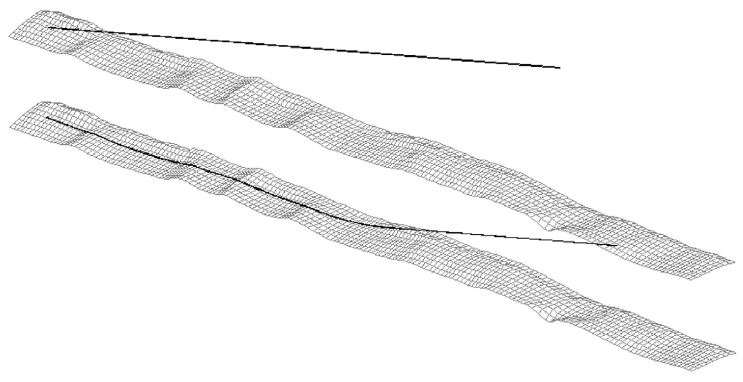
\includegraphics[width=0.7\linewidth]{imagens/lancamento_do_duto}
    \caption[]{Modelo de elementos finitos durante o lançamento.\\Fonte:~\cite{Bai2014}}\label{fig:lancamentododuto}
\end{figure}

Por simplicidade, neste trabalho, será assumido que o ângulo entre o duto e a horizontal o será nulo, isto é, o duto estará num plano horizontal que desce em direção a superfície batimétrica.
Desso modo, o modelo permitirá especificar somente a tração de lançamento.
Essa modelagem visa garantir a correta representação do contato entre o duto e a batimetria (forças de contato e ponto onde o duto toca o solo).
A Figura~\ref{fig:lancamentododuto} mostra o duto antes e durante o processo de instalação.

A medida que o duto se assenta é necessário garantir um equilíbrio estável entre o duto e o solo, o que é feito mediante um modelo representativo dessa iteração, no qual deve-se definir o atrito e rigidez do leito marinho.
No \abaqus~\cite{Dassault2018}, pode-ser relacionar a penetração e a pressão de resposta do solo por meio de uma curva de rigidez axial, além de usar modelo anisotrópico para o atrito do solo para representar as diferenças entre os atritos nas direções longitudinal e transversal.

Após a descida do duto, tem-se os processos de alagamento e desalagamento, que acarreta em mudanças no peso submerso do duto e, consequentemente, altera na sua configuração.
Esses processos podem ser facilmente modelados por uma variação numa carga vertical atuando no duto.
Mas, um duto sujeito a essa variação de carga na condição alagada sofrem grandes deformações axiais devido à mudança em geometria, e assim o duto se deforma e afunda nos vãos livres ao longo da rota do duto, como mostra a \autoref{fig:duto_alagado}.

\begin{figure}[th!]
    \centering
    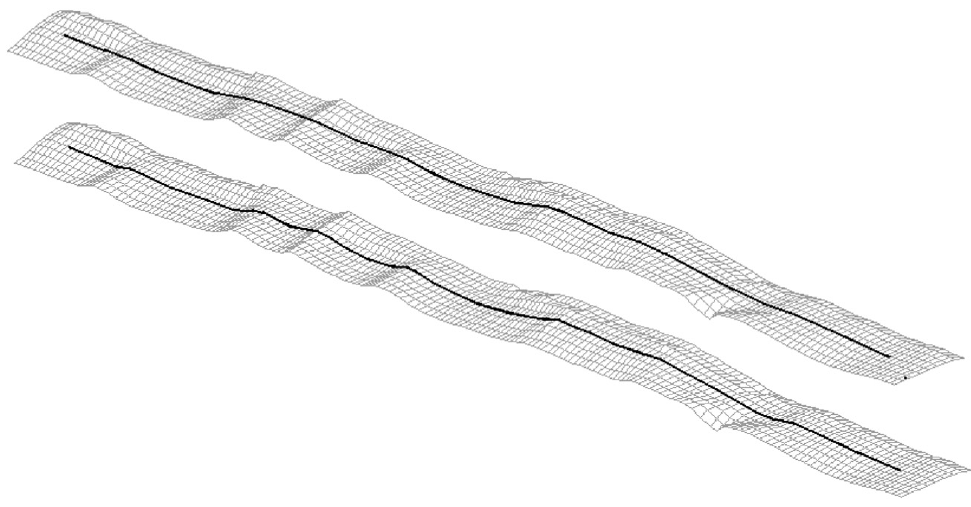
\includegraphics[width=0.7\linewidth]{imagens/duto_alagado}
    \caption[]{Modelo com o duto vazio (acima) e alagado (abaixo).\\Fonte:~\cite{Ose1999}}\label{fig:duto_alagado}
\end{figure}

Dessa maneira, é desejável que o modelo a ser estabelecido use um procedimento de análise que considere grandes deslocamentos e o efeito de alterações na área da seção do duto devido a alta tensão axial.
Além disso, é interessante qu eo modelo de material seja capaz de representar o comportamento plástico da seção do duto. No trabalho aqui proposto, não serão contempladas nas análises envolvendo efeitos de carregamentos de temperatura.

A pressão hidrostática externa é um fator importante para a capacidade de resistência de duto em águas profundas.
Como o modelo pode incluir uma estrutura tridimensional no fundo do mar, a pressão externa pode ser uma função da profundidade da água.
Já a pressão interna pode ser assumida como constante, mas a possibilidade de representar o efeito estática do conteúdo na extremidade pode ser incluído.


\section{Procedimentos e etapas de carregamento na análise de elementos finitos}


Um conceito base no \abaqus~é a divisão do histórico do cargamentos em etapas de carga. Para cada etapa, o usuário escolhe um método de análise.
Dessa forma, é possível representar qualquer sequência  e tipo de histórico de carregamento.
Por exemplo, em um passo estático, o duto pode ser carregado com gás, no passo estático seguinte descarregado, e na terceira etapa, pode-se realizar uma análise exclusiva do duto vazio.
Um histórico de carga de um modelo construído para análise é apresentado na~\autoref{tab:load_steps}.


\begin{table}[!ht]
\renewcommand{\arraystretch}{1.2}
\small
\centering
\caption[]{Histórico de carga típico em uma análise de dutos no ABAQUS.}
\label{tab:load_steps}
\begin{tabular}{cll}
\toprule[1.5pt]

\textbf{Passo} & \textbf{Ação} & \textbf{Análise} \\
\midrule
1 & Aplicação de peso próprio e empuxo do duto & Estática \\
2 & Aplicação de pressão externa hidrostática & Estática \\
3 & Aplicação de tensão leiga & Estática \\
4 & Assentamento do duto no fundo do mar (ver \autoref{fig:lancamentododuto}) & Estática \\
5 & Remoção dos elementos de guincho & Estática \\
6 & Modificando condições de contorno para a condição de instalação & Estática \\
7 & Enchimento de água para condições alagadas (ver \autoref{fig:duto_alagado}) & Estática \\
8 & Aplicação de pressão do teste hidrostático. & Estática \\
9 & Remoção da pressão do teste hidrostático & Estática \\
10 & Enchimento de gás & Estática \\
11 & Aplicação de pressão de operação & Estática \\
12 & Aplicação de temperatura de operação para a condição operacional & Estática \\
13 & Remoção de pressão e temperatura para condição de recarga & Estática \\
14 & Aplicação de carga de onda e corrente & Dinâmica \\

\bottomrule[1.25pt]
\end{tabular}
\\[6pt]
Fonte: \citeonline{Bai2014}
\end{table}

É válido de nota que a análise estática disponível no ABAQUS usada no modelo lida com respostas não lineares de efeitos de grandes deslocamentos, não-linearidade do material e não-linearidades de contorno, como contato, deslizamento e atrito (interação solo-duto). O ABAQUS usa o método de Newton para resolver as equações de equilíbrio não lineares. Portanto, a solução é obtida como uma série de incrementos com iterações para obter equilíbrio dentro de cada incremento \cite{SIMULIA2018}.

\section{Tipos de elementos}

O Abaqus dispõe de alguns tipos de elementos a serem usados no modelo do sistema de solo-duto com elementos finitos, conforme a \autoref{fig:elements_type}:

\begin{itemize}
    \item Para modelar o fundo do mar pode-ser usar os elementos rígidos do tipo R3D4 usados, ou superfícies analíticas rígidas.
    \item Os elementos do tipo PIPE31H usados para modelar o duto.
    \item Os elementos de molas usados para representar a continuidade do duto nas extremidades.
\end{itemize}

\begin{figure}[th!]
    \centering
    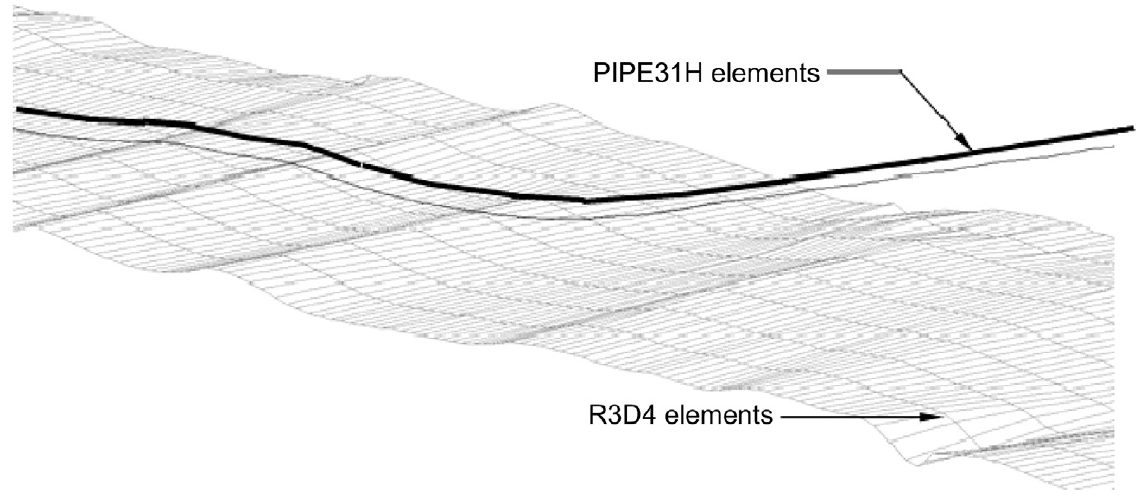
\includegraphics[width=0.8\linewidth]{imagens/elements_types}
    \caption[]{Tipos de elementos usados no modelo.\\Fonte:~\cite{Bai2014}}\label{fig:elements_type}
\end{figure}

\subsection{Elemento PIPE31/PIPE32}

A \autoref{fig:elemen_PIPE31H} mostra o elemento de duto finito 3D usado no modelo estabelecido, com 2 nós e 12 graus de liberdade.
O elemento PIPE31 usa interpolação linear, e o elemento PIPE32 interpolação quadrática.
A formulação híbrida torna o elemento adequado para casos com estruturas delgadas e problemas de contato, como um duto descendo sobre o fundo do mar.

Os elementos híbridos (PIPE31H/PIPE32H) são fornecidos para uso nos casos em que é numericamente difícil calcular as forças axiais e de cisalhamento pelo método de deslocamento próprio do Método dos Elementos Finitos.
O problema nesses casos é que pequenas diferenças em posições nodais podem causar forças muito grandes em algumas partes do modelo, o que por sua vez, causar grandes deslocamentos em outras direções.
Os elementos híbridos superam essa dificuldade usando uma formulação mais geral, na qual as forças de cisalhamento axial e transversal nos elementos são incluídas, juntamente com os deslocamentos e rotações nodais, como variáveis primárias.
Embora essa formulação torne esses elementos mais custosos computacionalmente, eles geralmente convergem muito mais rapidamente quando as rotações dos dutos são grandes.

O elemento está disponível com uma seção circular vazada de paredes finas e suporta a possibilidade de o usuário especificar pressão externa ou interna.
Elementos de paredes espessas também estão incluídos no ABAQUS.
O elemento também pode considerar alterações na área da seção do duto devido ao alto nível tensão axial do duto.

\begin{figure}[!ht]
    \centering
    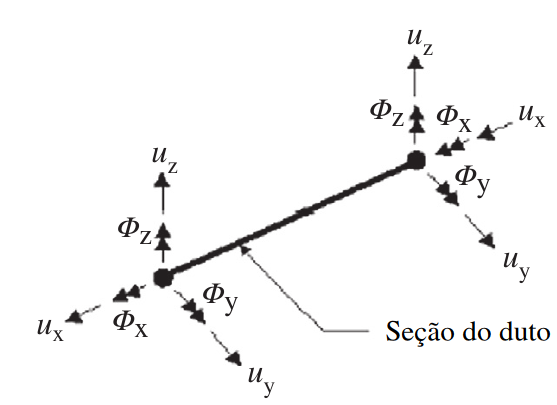
\includegraphics[width=0.5\linewidth]{imagens/elemen_PIPE31H}
    \caption[]{Elemento PIPE31.\\Fonte:~\cite{Bai2014}}\label{fig:elemen_PIPE31H}
\end{figure}

\subsection{Elemento R3D4}

O elemento rígido R3D4 de quatro nós, como mostrado na \autoref{fig:element_R3D4}, possibilita modelar superfícies complexas com geometria arbitrária e é geralmente escolhido ao modelar a topografia do fundo do mar. Uma característica muito importante do ABAQUS ao modelar o fundo do mar tem sido a possibilidade de suavizar as superfícies geradas com os elementos rígidos, o que leva a uma representação muito melhor do fundo do mar do que a superfície facetada inicial.

\begin{figure}[th!]
    \centering
    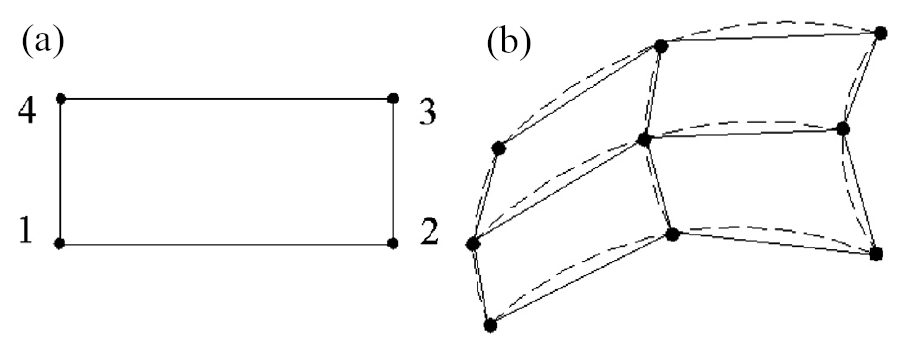
\includegraphics[width=0.7\linewidth]{imagens/element_R3D4}
    \caption[]{Elemento rígido R3D4 (a), e suavização da superfície superfície de elementos (b).\\Fonte:~\cite{Bai2014}}\label{fig:element_R3D4}
\end{figure}

A suavização é feita pela ABAQUS, criando superfícies de Bèzier com base na superfície facetada do fundo do mar formada pelos elementos rígidos. As superfícies de Bèzier resultantes, diferentemente da superfície do elemento facetado, são lisas e têm uma superfície externa com direção normal contínua. As superfícies de Bèzier não correspondem exatamente à geometria facetada da superfície rígida, mas os nós dos elementos rígidos que definem o fundo do mar permanecem sempre na superfície de Bèzier. Além disso, o usuário pode especificar o grau de suavização para controlar a geometria da superfície suavizada.

Um conjunto de elementos R3D4 que definem o fundo do mar é usado como a superfície principal chamada para aplicações de contato com os elementos do duto. Isso significa que um par de contatos (solo-duto) é definido e um modelo de interação é especificado. Esse modelo de interação geralmente consiste em uma definição de rigidez e atrito no fundo do mar.


\subsection{Superfície analítica rígida}

Outra forma deb representar a batimetria do piso marinho é utilizar uma superfície analítica rígida, isto é, uma superfície geométrica com perfis que podem ser descritos com segmentos de linha reta ou curva. Estes perfis podem ser varridos por um vetor gerador ou rotacionados em relação a um eixo para formar uma superfície tridimensional. Uma superfície analítica rígida está associada a um nó de referência de corpo rígido, cujo movimento governa toda a superfície. É importante frisar que este tipo de superfície possui apenas um lado disponível para contato, especificado de acordo com a orientação de eixos definida.

Em relação ao uso de superfícies formadas por elementos, o uso de superfícies analíticas rígidas apresenta duas vantagens:
\begin{itemize}
    \item Superfícies geométricas curvas podem ser modeladas com precisão, uma vez que é possível parametrizá-las com segmentos de linhas curvas, o que tem como resultado uma superfície mais suave, fornecendo uma melhor aproximação à restrição de contato físico.
    \item Menor custo computacional decorrente do algoritmo de contato.
\end{itemize}

Por outro lado, como desvantagens do uso deste tipo de superfície:
\begin{itemize}
    \item Uma superfície analítica rígida sempre agirá como superfície \textit{master} em uma interação de contato, impossibilitando que se modele o contato entre duas superfícies rígidas analíticas.
    \item Forças de contato e pressões não podem ser plotadas em uma superfície rígida analítica, apenas na superfície \textit{slave}.
    \item Um número muito grande de segmentos, na ordem de milhares, para definir uma superfície rígida analítica pode diminuir o desempenho. Sendo mais recomendável o uso de superfícies baseadas em elementos.
\end{itemize}


Para os casos estudados, utilizou-se uma superfície cilíndrica rígida tridimensional, conforme Figura~\ref{fig:superficie_analitica}. Para criação desta superfície é necessário fixar os pontos que definem um sistema de coordenadas locais, \textbf{a}, \textbf{b} e \textbf{c}. As coordenadas destes pontos, $(X_a, Y_a, Z_a)$, $(X_b, Y_b, Z_b)$ e $(X_c, Y_c, Z_c)$, são dadas em relação ao sistema de coordenas global. O ponto \textbf{a} define a origem do sistema de coordenadas local; o ponto \textbf{b} define o eixo-$x$ local e o ponto \textbf{c}, que se refere ao eixo-$z$ local negativo, define o vetor de geração.  Portanto, os segmentos que formam o perfil da superfície rígida são definidos no eixo $x$-$y$ local e a superfície rígida tridimensional, de acordo com o vetor de geração.

\begin{figure}[!ht]
    \centering
    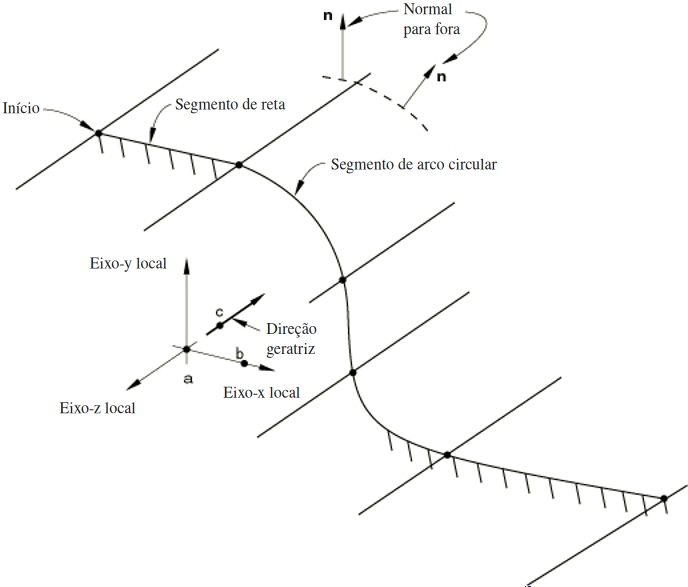
\includegraphics[width=0.7\textwidth]{imagens/superficie_analitica}
    \caption[]{\label{fig:superficie_analitica} Exemplo de superfície analítica rígida.\\Fonte: \citeonline{SIMULIA2018}}
\end{figure}

%\chapter{Desenvolvimento da ferramenta}\label{chap:software}

% Isto está de acordo com o que comentei anteriormente. Este levantamento deve ser uma das etapas importantes de sua metodologia.

O levantamento dos requisitos de um sistema é o processo que fornece os subsídios que devem nortear uma série de decisões a serem tomadas no seu desenvolvimento. Primeiramente, apresenta-se aqui o fluxo de trabalho tradicional para análise de fadiga de um duto em vão livre. % TODO Aqui eu faria uma descrição sucinta das etapas associadas a este levantamento dos requisitos. Cada etapa seria uma subseção.

\section{Fluxo de avaliação de vida à fadiga sem o \frame}\label{sec:workflow}


Baseado nos estudos e oficinas realizados para o desenvolvimento deste trabalho. Pôde-se estabelecer que a análise de vida à fadiga em dutos em vão-livre compreende o fluxograma apresentado na \autoref{fig:fluxograma}. % chktex 19

\begin{figure}[!ht]
    \centering
    \caption{Fluxo de avaliação de vida à fadiga em dutos em vão-livre.}\label{fig:fluxograma}
    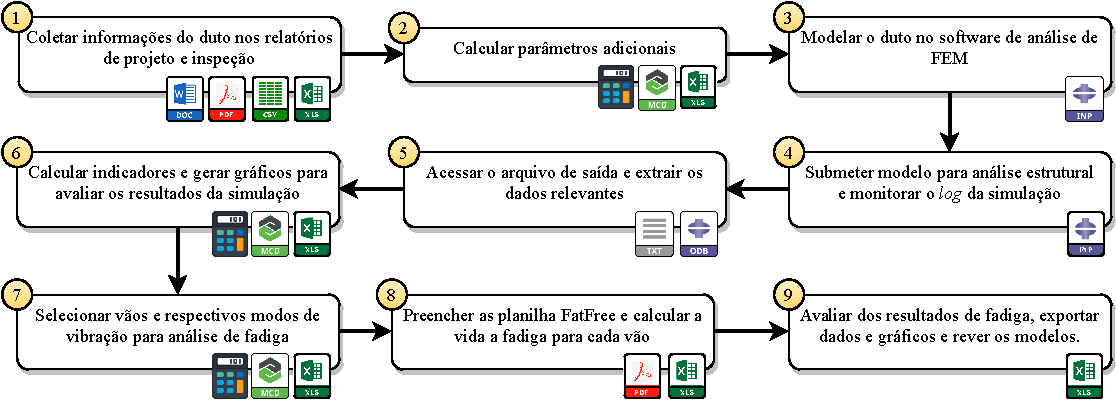
\includegraphics[width=\textwidth]{imagens/fluxograma.pdf}
    \fonte{Autor (2020)}
\end{figure}

A seguir, uma breve descrição de cada item:

\begin{enumerate}[label= (\arabic*)]
    \item Nesta etapa, o profissional reúne as informações básicas para construção dos modelos e outros dados usados em cálculos posteriores. Citadamente, temos aqui: as cotas do perfil do duto e batimetria obtidas na inspeção, geometria e propriedades dos materiais das camadas que compõem sessão do duto, parâmetros do solo, coeficientes de segurança e outras constantes físicas, posição e tipos de suportes ao longo do duto. Essa tarefa envole analisar uma série de documentos (\texttt{.doc}, \texttt{.pdf}, etc) em busca desses valores, dispostos de forma não estruturada. Quando estruturados, em forma de arquivos CSV ou planilhas, por exemplo, é necessário ainda manipular esses dados de modo a extrair somente a informação necessária e/ou convertê-las no formato apropriado. Um exemplo disso são os dados de batimetria, que precisam convertidos nas coordenadas dos nós de uma malha de elementos finitos no formato de um arquivo \texttt{.inp}.---no caso do ABAQUS. De posse desses dados, pode-se então, iniciar a fase de pré-processamento.
    \item Uma vez que nem todos os dados a serem utilizados estão de acordo com as especificações dos softwares a serem empregados nas análises numéricas, ainda é necessários manipular alguns desses valores, seja calculando constantes ou convertendo unidades. Para isso, geralmente utiliza-se softwares de planilhas e/ou folhas de cálculos (Microsoft Excel, MathCad, Maple, etc.). Esta etapa inicia o pré-processamento dos dados.
    \item Com todos os dados em mãos, é necessário transformá-los em um modelo no software de elementos finitos, via interação com mouse e teclado (GUI), ou criando arquivos de entrada. Embora a reutilização de arquivos de entrada previamente criados facilite essa tarefa, nem todos os trechos desses arquivos são suficientes ou podem ser reaproveitados. Estas limitações são frequentes em trechos do arquivo que precisam ser repetidos a depender da quantidade de certas entidades no modelo---suportes, por exemplo. Ao fim desta etapa, encerra-se o pré-processamento dos dados.
    \item Por mais simples que seja submeter o modelo para análise na maioria dos softwares de análise de elementos (alguns cliques via GUI, ou um comando via CLI\footnote{\textit{Command Line Interface}: interface de linha de comando}), as análises costumam levar horas e envolver execuções sucessivas a fim de realizar intervenções no modelo que não podem ser modeladas previamente. Dessa forma, torna-se necessário o monitoramento do progresso da simulação. Esta etapa compreende a primeira parte do processamento propriamente dito.
    \item Uma vez concluída a simulação Análise de Elementos Finitos (FEA, em inglês), é necessário analisar os resultados antes do pós-processamento. Por vezes, é preciso extrair os resultados que estão armazenados em arquivos proprietários (como \texttt{.odb}, no caso do ABAQUS), utilizando as funcionalidades das ferramentas dos próprios pacotes de software de elementos finitos para isso. Esta tarefa, geralmente feita via GUI, costuma ser repetitiva e pode levar de alguns minutos ou horas. Esta etapa inicia parte do pós-processamento da FEA\@.
    \item De posse dos resultados em formatos acessíveis a outros software (MS Excel e MathCad, por exemplo), é necessário calcular (e muitas vezes visualizar em gráficos) alguns indicadores a fim de avaliar a validade dos resultados. Embora poderosos, estes softwares ainda carecem de gráficos mais interativos, como possibilidades de ampliar e transladar os gráficos com o mouse. Esta etapa encerra o pós-processamento da FEA\@.
    \item Na metodologia presente na \dnvf105---que será abordada adiante no \autoref{sec:multimode}---o cálculo de fadiga é baseada em modelos de resposta, portanto, é necessário calcular a resposta de cada modo para as várias condições de carregamento ambiental, o que a torna impraticável sem automação. Para solucionar este problema, foi criada a \fatfree, uma planilha de cálculo comercial que realiza estas operações. No entanto, dentre as dezenas de modos obtidos por solução modal na FEA costumam aparecer modos espúrios. Dessa forma, antes de realizar a análise na \fatfree, é necessário escolher dentre os modos de vibração obtidos na simulação numérica aqueles que mais contribuem para fadiga. Esta tarefa pode ser feita via inspeção visual, observando a forma dos modos, mas é uma prática pouco precisa e subjetiva.
    \item Uma vez selecionados os modos a serem usados para cálculo de fadiga, é necessário o preenchimento da planilha com os dados de deflexão normalizada de cada modos, o que consiste em algumas centenas de valores. Além disso, é necessário preencher muitas outras informações referentes geometria e propriedades dos materiais da sessão do duto, parâmetros do solo, coeficientes de segurança e condições de carregamento em várias páginas diferentes. Com todos os dados preenchidos e opções selecionadas nos controles da planilha, pode-se apertar o botão que calcula os resultados de fadiga.
    \item Finalmente, os dados de fadiga pode ser analisados e exportados para outras ferramentas a fim de gerar relatórios.
\end{enumerate}


\section{Fluxo de avaliação de vida à fadiga com uso da ferramenta} % TODO Seria importante apresentar este fluxo de uma forma mais conceitual, sem ser específico no uso do ABAQUS ou FatFree. Quando for necessário comentar sobre essas ferramentas, poderia fazer isto citando-as como exemplos do fluxo conceitual.


A ferramenta proposta tem como requisito atender o fluxo apresentado na \autoref{sec:workflow}, automatizando certas etapas da análise de vida à fadiga. Os itens 1, 3, 4 e 6 são cobertos pela implementação ferramenta, e os itens 2 e 5 são realizados em aplicações externas.

% TODO Seria muito legal ver esse fluxo usando o framework de uma forma conceitual e global, sem se restringir a softwares específicos. Para integrar um simulador de EF, por exemplo, talvez fosse necessário atender algum protocolo que o seu framework iria estabelecer. Isto ficaria muito legal e independente de aplicações externas específicas.

\begin{figure}[!ht]
    \centering
    \caption{Fluxo de operação proposto para a ferramenta.}\label{fig:workflow}
    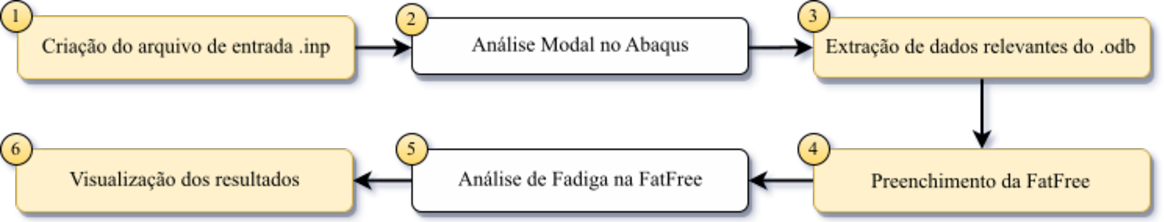
\includegraphics[width=\textwidth]{imagens/fluxograma_automatizado}
\end{figure}

De forma mais detalhada, a ferramenta deve:


% TODO Como dito acima, eu esperava ver algo mais conceitual, sem uma dependência de softwares externos específicos. Seria importante aqui estabelecer os protocolos de comunicação entre o framework e seus plugins (que seriam os softwares externos). Eu e Setton fizemos isto em nosso mestrado. Trabalhamos no desenvolvimento de um sistema para gerenciamento de atributos que poderia ser integrado a qualquer pré-processador de elementos finitos.

\begin{enumerate}[label= (\arabic*)]
    \item A partir de um arquivo de entrada com informações do modelo, criar arquivos de entrada para o ABAQUS (.inp) que reproduza todo o processo de simulação do comportamento do duto apresentado (\autoref{sec:assentamento});
    \item Submeter o arquivo gerado para análise no ABAQUS. No caso de haver um passo de caraga para a colocação de suportes, a simulação é executada em duas partes:
    \begin{enumerate}
        \item a primeira com os passos de carga anteriores a colocação dos suportes, e
        \item a segunda com o passo da colocação dos suportes e os passos de carga seguintes.
    \end{enumerate}
    \item Processar os arquivos de saída do ABAQUS (.odb) extraindo as informações relevantes como a configuração deformada, modos de vibração, etc., gerando arquivos em outros formatos de fácil leitura para pós-processamento, tanto por este \frame, quanto por outros softwares;
    \item Pós-processar as informações gerando gráficos e relatórios relevantes para as tomadas de decisão do usuário. Esse é o requisito mais crítico, uma vez que é fundamental o entendimento sobre a análise de duto em vão-livre. Entre as tarefas que fazem parte deste item está a automação da escolha dos modos de vibração ativos e relevantes e para cada vão de interesse (a qual deve ser norteada pelos aspectos discutidos na \autoref{sec:multimode}) e a manipulação da FatFree;
    \item Ativar o processo de cálculo de fadiga no arquivo da FatFree preenchido no passo anterior;
    \item Capturar os resultados no arquivo \texttt{.xls} da \fatfree, que agora contém os resultados do cálculo de vida à fadiga, e apresentá-los na forma de gráficos e relatórios.
\end{enumerate}


\section{Implementação computacional}

% TODO: nunca deixa uma seção vazia dessa forma, ao menos apresente o que. vem dentro dela, de forma resumida.

\subsection{Linguagem de programação}\label{sec:python}

Python\footnote{https://www.python.org} foi a linguagem de programação adotada para implementação da ferramenta. Além de ser uma linguagem interpretada de alto nível Orientada a Objeto --- que permite um alto índice de reaproveitamento de código --- e da sintaxe simples. \citeonline{Rao2018} apresenta algumas das principais vantagens que destaca a linguagem para este tipo de aplicação:

\begin{itemize}
    \item Disponibilidade de bibliotecas para aplicações científicas contemplando manipulação de matrizes (Numpy), funções matemáticas (SciPy), manipulação de dados em forma tabular (Pandas), criação de gráficos interativos (Matplotlib e Bokeh);

    \item Suporte para automação de tarefas. Os recursos de \textit{script} internos do Python e vários pacotes têm um forte suporte à automação de tarefas. A automação de tarefas repetitivas e a realização do registro de dados são fáceis e requerem pouco esforço. O ABAQUS, por exemplo, permite modelagem e acesso a informações em arquivos de saída via Python. A biblioteca xlwings permite manipulação de planilhas Excel, a exemplo da FatFree;

    \item Pacotes Python como Django e Flask tornam possível desenvolver e usar o Python como uma API\footnote{Na programação de computadores, uma Interface de Programação de Aplicativos (\textit{Application Programming Interface} --- API) é um conjunto de definições de sub-rotinas e ferramentas para a criação de software. Em termos gerais, é um conjunto de métodos de comunicação claramente definidos entre vários componentes.} com um \textit{front-end} da web. Essa funcionalidade é particularmente útil para reaproveitamento da ferramenta  em outras aplicações.
\end{itemize}


\subsection{Pacotes e classes}


Para implementação do fluxo de trabalho proposto para a ferramenta, fez-se a implementação de módulos para lidar com cada contexto específico.
Em python, módulos podem ser quaisquer arquivos com extensão \texttt{.py}.
Estes módulos podem ser agrupados em pacotes, que são pastas que, além dos módulos, contém um arquivo \texttt{\_\_init\_\_.py}.  % chktex 21
Na ferramenta, têm-se alguns pacotes que agrupam módulos em torno do contexto de um problema que o \textit{software} resolve.


\subsubsection{Pacote \texttt{analysis}}


É o pacote principal responsável por orquestrar o fluxo de trabalho da ferramenta desde o processamento dos dados de entrada, geração dos arquivos para o ABAQUS e os pós-processamentos.
As funções de pré-processamento de dados estão aqui.
Este pacote tem dois módulos (\texttt{models.py} e \texttt{inp.py}) que contém duas classes principais, respectivamente:

\begin{itemize}
    \item \texttt{Model}: classe que contém as informações do modelo do problema.
    A classe armazena todas as informações para construção dos arquivos \texttt{.inp}, isto é, dados de batimetria, material, geometria do duto, coeficientes de segurança, entre outros.
    A principal forma de criação da instâncias dessa classe é pelo método estático \texttt{load\_json}, que recebe um arquivo principal de entrada (em formato JSON, ver \autoref{apendice:json}), e realiza o pré-processamento dos dados contidos nele;

    \item \texttt{Inp}: lida com a escrita modularizada de arquivos de entrada  para o ABAQUS. Tem-se um arquivo \texttt{.inp} principal que conterá informações para a localização de outros arquivos acessórios que, por sua vez, terão as informações específicas de cada aspecto da modelagem: batimetria, passos de carga, etc. Isso facilita o reaproveitamento dos arquivos acessórios, sem a necessidade de alterações no arquivo principal.
\end{itemize}

Na \autoref{fig:analysis-uml} vê-se um diagrama UML\footnote{Sigla para \textit{Unified Modeling Language}: Linguagem Unificada de Modelagem é uma linguagem padrão para modelagem orientada a objetos~\cite{infoescolauml}} com uma visão geral do pacote \texttt{analysis}.

\begin{figure}[!ht]
    \centering
    \caption{Digrama UML do pacote \texttt{analysis}.}\label{fig:analysis-uml}
    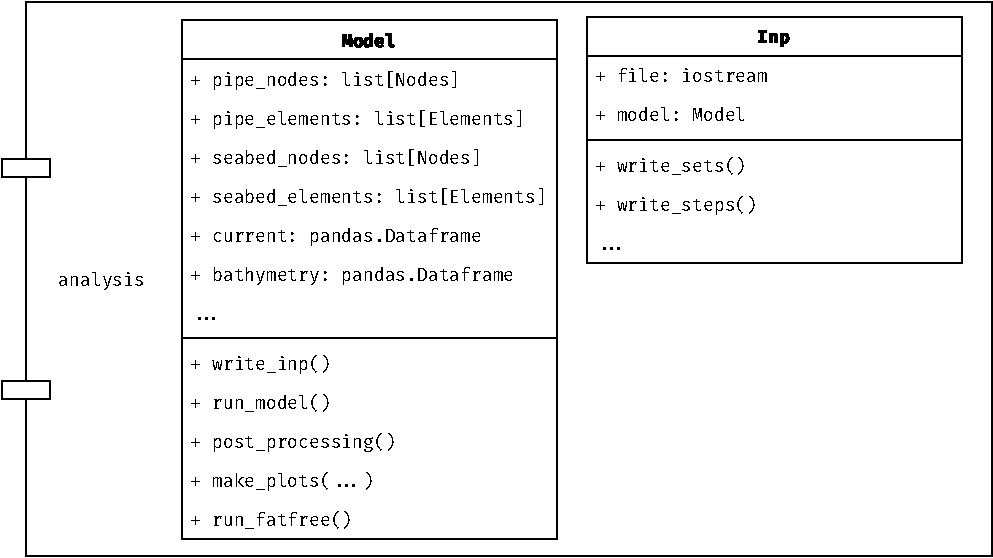
\includegraphics[width=0.8\textwidth]{imagens/analysis-uml}
    \fonte{Autor (2020)}
\end{figure}


\subsubsection{Pacote \texttt{odb\_handler}}


Neste pacote está o módulo responsável por lidar com os arquivos de saída do ABAQUS (odb) no sentido de acessar e guardar os dados relevantes em arquivos com formatos de fácil manipulação por outros softwares (CSV e JSON, por exemplo, que possui módulos para leitura e escrita nativos em Python).

Na \autoref{fig:odb-handler-uml} vê-se um diagrama UML com uma visão geral do pacote \texttt{odb\_handler}.

\begin{figure}[!ht]
    \centering
    \caption{Digrama UML do pacote \texttt{odb\_handler}.}\label{fig:odb-handler-uml}
    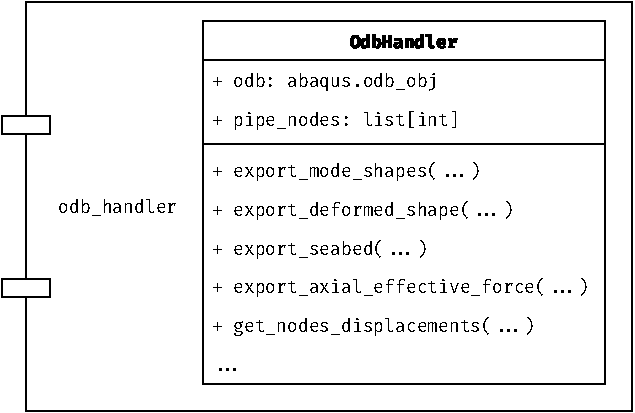
\includegraphics[width=0.5\textwidth]{imagens/odb-handler-uml}
    \fonte{Autor (2020)}
\end{figure}


\subsubsection{Pacote \texttt{mode\_selector}}


Neste pacote estão implementados os métodos responsáveis pela estratégia de seleção automática de modos de vibração (que depende da definição dos vãos), bem como a manipulação dos dados associados aos vãos e seus respectivos modos. As abstrações dos conceitos de vão e modo de vibração estão implementadas nas seguintes classes:

\begin{itemize}
    \item \texttt{Span}: classe que representa um vão do duto. Uma vez que análise de fadiga é feita por vão, é nessa classe que são implementados os métodos responsáveis pela seleção dos modos de vibração, que são ligados à classe por um dos seus atributos;

    \item \texttt{ModeShape}: classe que representa um modo de vibração (\textit{mode shape}). A principal forma de criação de objetos dessa classe é por meio da função \texttt{load\_json} do módulo \texttt{mode\_shapes.py}, que carrega os dados do arquivo gerado com utilização do \texttt{odb\_handler}, e retorna uma lista de objetos desta classe.
\end{itemize}

Na \autoref{fig:mode-selector-uml} vê-se um diagrama UML com uma visão geral do pacote \texttt{mode\_selector}.

\begin{figure}[!ht]
    \centering
    \caption{Digrama UML do pacote \texttt{mode\_selector}.}\label{fig:mode-selector-uml}
    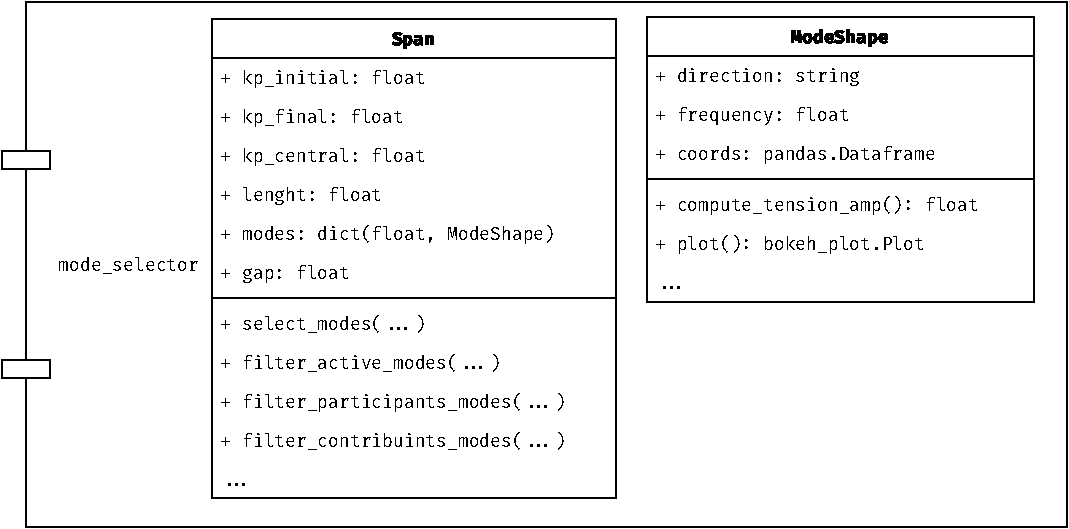
\includegraphics[width=0.8\textwidth]{imagens/mode-selector-uml}
    \fonte{Autor (2020)}
\end{figure}


\subsubsection{Pacote \texttt{dnv}}

Neste pacote são agrupadas módulos referentes à \dnvf105, como cálculos dos modelos de resposta da \dnvf105, que alimentam o algoritmo de seleção de modos de vibração, e entrada de saída de dados da planilha FatFree. As principais classes contidas nesses pacotes são:

\begin{itemize}
    \item \texttt{ResponseModel}: implementa a formulação dos modelos de resposta apresentados na \autoref{sec:viv};

    \item \texttt{FatFree}: responsável por fazer a entrada dos dados na planilha e invocar a execução dos cálculos. Essa classe faz uso da biblioteca \texttt{Xlwings}, que consegue se comunicar com o Microsoft Excel e manipular os componentes (caixas de seleção, botões, etc) que formam a interface da FatFree;

    \item \texttt{FatFreeResults}: esta classe permite o acesso facilitado aos dados contidos em um determinado arquivo da FatFree.
\end{itemize}

Na \autoref{fig:dnv-uml} vê-se um diagrama UML com uma visão geral do pacote \texttt{dnv}.

\begin{figure}[!ht]
    \centering
    \caption{Digrama UML do pacote \texttt{dnv}.}\label{fig:dnv-uml}
    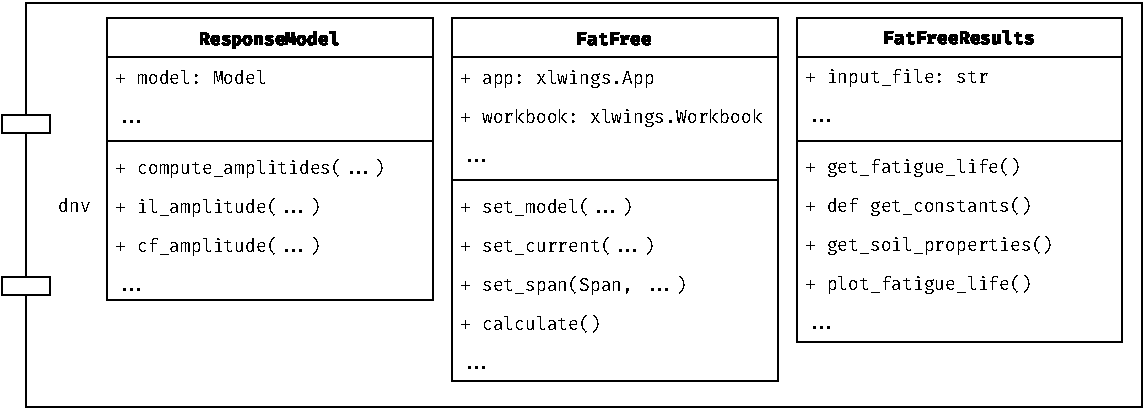
\includegraphics[width=\textwidth]{imagens/dnv-uml}
    \fonte{Autor (2020)}
\end{figure}


\subsubsection{Pacote \texttt{plots}}


Pacote responsável por agregar as funções de geração de gráficos dos resultados. Disponibilizar essas funções como parte da ferramenta permite que os gráficos com os resultados das análises sejam gerados automaticamente, além de padronizar o visual e a forma de apresentação. As principais classes neste pacote são:

\begin{itemize}

    \item \texttt{Plot}: é construída em cima da classe \texttt{Figure} da biblioteca \texttt{Bokeh}\footnote{www.bokeh.org}, que permite a criação de gráficos interativos em HMTL. Os gráficos gerados por essa biblioteca possuem controles que permitem, por exemplo, que o usuário dê zoom ou translade os dados exibidos, ative/desative os itens mostrados por meio de clique nos respectivos itens nas legendas, salve o gráfico em formato de imagem estática (\texttt{png}). Na \autoref{fig:exemplo-bokeh} vê-se um exemplo desses gráficos, destacando os elementos interativos em vermelho;

    \begin{figure}[!ht]
        \centering
        \caption{Exemplo de gráfico customizado criado com a biblioteca Bokeh.}\label{fig:exemplo-bokeh}
        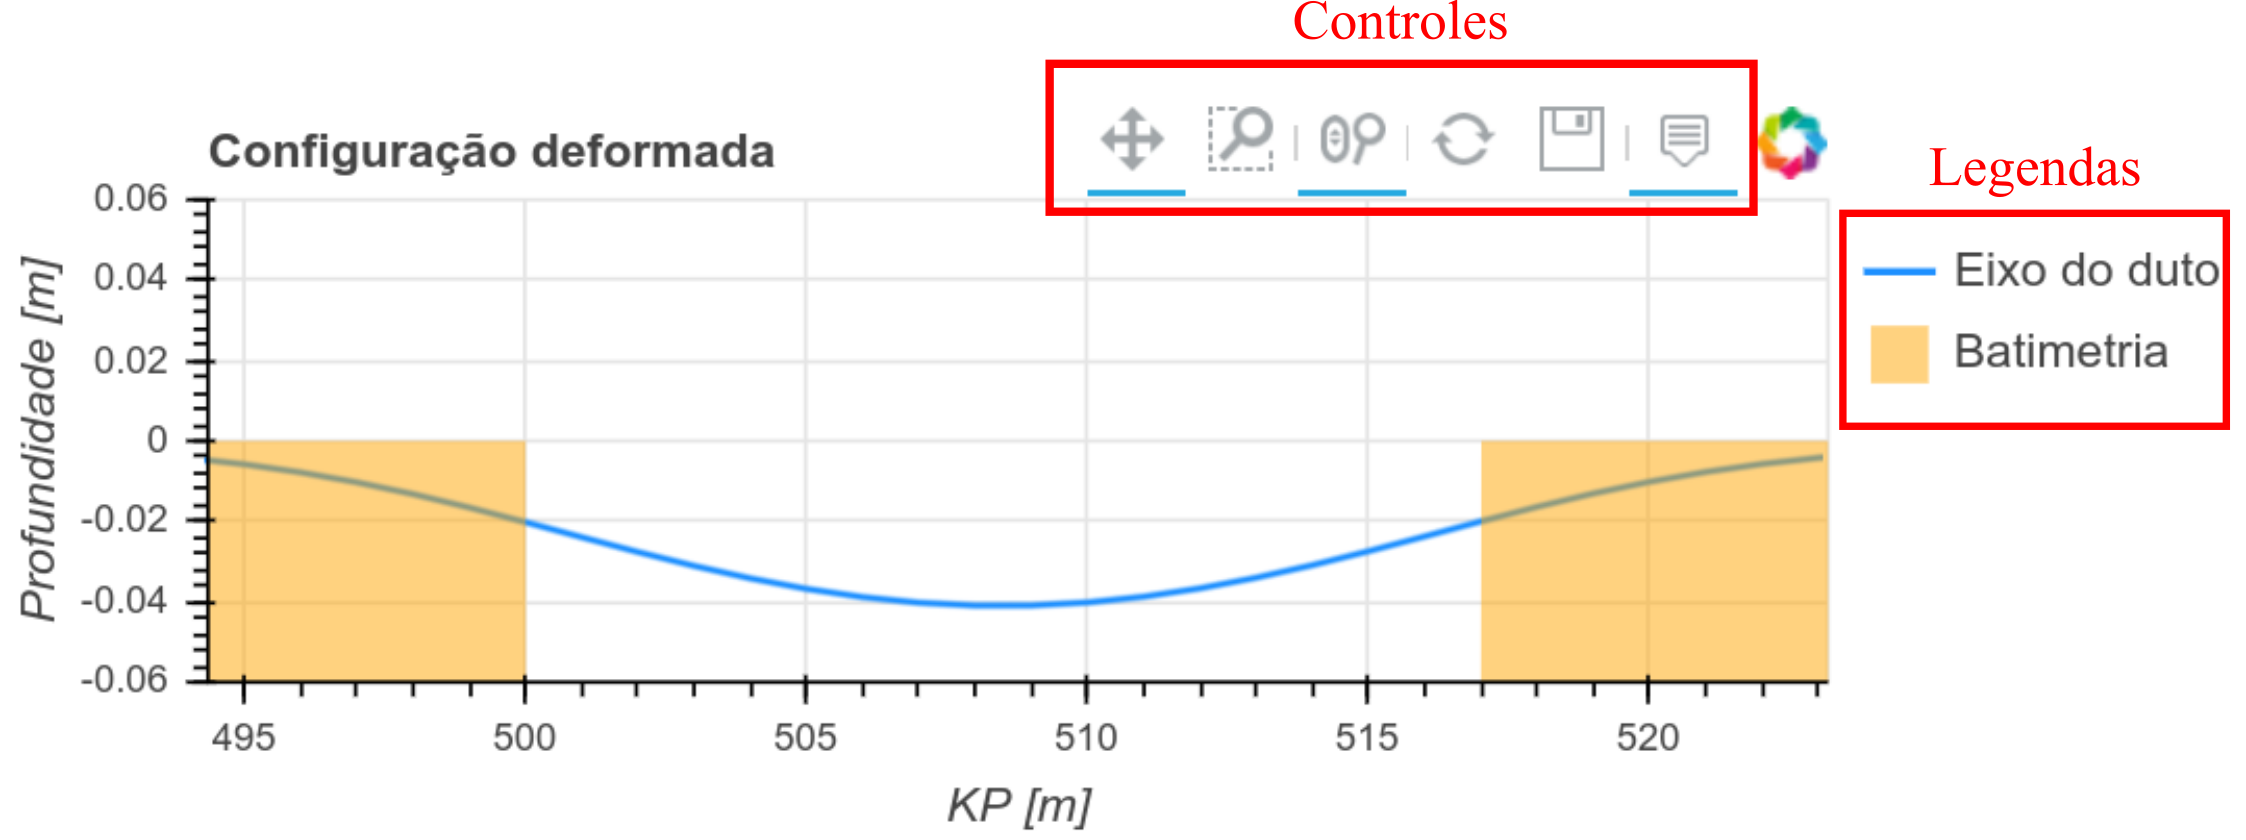
\includegraphics[width=0.8\textwidth]{imagens/exemplo-bokeh}
        \fonte{Autor (2020)}
    \end{figure}

    O objetivo da classe \texttt{Plot} é simplificar a criação dos gráficos devido a implementação de métodos que facilitam desde alterar os componentes mais comuns das figuras, como títulos dos eixos e legendas, até combinar gráficos e formar \textit{dashboards} com gráficos integrados. A combinação de gráficos pode ser feita por meio dos operadores matemáticos:
    \begin{itemize}
        \item \texttt{a + b}: para sobrepor os gráficos \texttt{a} e \texttt{b};
        \item \texttt{a | b}: para posicionar dois gráficos, com \texttt{a} à esquerda de \texttt{b};
        \item \texttt{a / b}: para posicionar dois gráficos, com \texttt{a} acima de \texttt{b};
    \end{itemize}

    \item \texttt{PipeProfileDashboards}: esta classe se utiliza da classe \texttt{Plot} para facilitar a criação de um tipo \textit{dashboard} recorrente no processo de análise: dois gráficos empilhados verticalmente, um com dados que podem ser associados a posição ao longo do duto (como esforço axial, modos de vibração, enterramento, vida à fadiga, etc), e o outro abaixo dele com o perfil do duto. Nesse tipo de arranjo é interessante que os eixos das abcissas estejam atrelados, permitindo ao usuário movimentar os dois eixos em sincronia.
\end{itemize}

Na \autoref{fig:plots-uml} vê-se um diagrama UML com uma visão geral do pacote \texttt{plots}.

\begin{figure}[!ht]
    \centering
    \caption{Digrama UML do pacote \texttt{plots}.}\label{fig:plots-uml}
    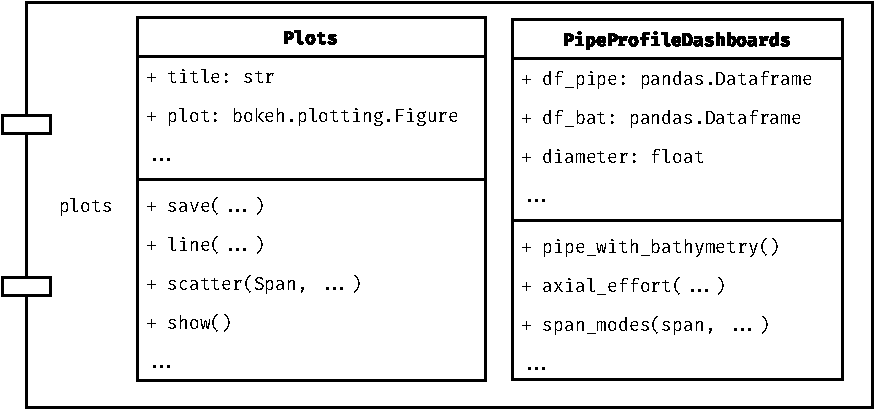
\includegraphics[width=0.7\textwidth]{imagens/plots-uml}
    \fonte{Autor (2020)}
\end{figure}

% TODO: O capítulo se encerrou sem um fechamento. Acho que falta algo. Outro detalhe: seria interessante um ou mais gráficos mostrando a relação entre essas classes. Acho que facilitaria o entendimento.

% ----------------------------------------------------------
% ELEMENTOS PÓS-TEXTUAIS (Referências, Glossário, Apêndices)
% ----------------------------------------------------------
\postextual

\bibliography{bibliografia}

\end{document}
